% This example is meant to be compiled with lualatex or xelatex
% The theme itself also supports pdflatex
\PassOptionsToPackage{unicode}{hyperref}
\documentclass[aspectratio=1610, xcolor=dvipsnames, 9pt]{beamer}

% Load packages you need here
\usepackage{polyglossia}
\setmainlanguage{german}

\usepackage{csquotes}
\usepackage{smartdiagram}

\usepackage{amsmath}
\usepackage{amssymb}
\usepackage{mathtools}

\usepackage{svg}
\usepackage{hyperref}
\usepackage{bookmark}
\usepackage{tikz}
\usepackage{graphicx}
\usetikzlibrary{shapes.geometric, arrows, positioning, shapes.geometric, calc}

\tikzstyle{process} = [rectangle, rounded corners, minimum width=3cm, minimum height=1cm, text centered, draw=black, fill=orange!50]
\tikzstyle{arrow} = [thick,->,>=stealth]

% load the theme after all packages

\usetheme[
  showtotalframes, % show total number of frames in the footline
]{fhswf}

% Put settings here, like
\unimathsetup{
  math-style=ISO,
  bold-style=ISO,
  nabla=upright,
  partial=upright,
  mathrm=sym,
}

\title{Advanced Natural Language Processing \& Large Language Models}
\author[F.~Neubürger]{ \textbf{Felix Neubürger}}
\institute[I \& W]{Fachhochschule Südwestfalen, Ingenieurs- \& Wirtschaftswissenschaften}
\date{2025}
\titlegraphic{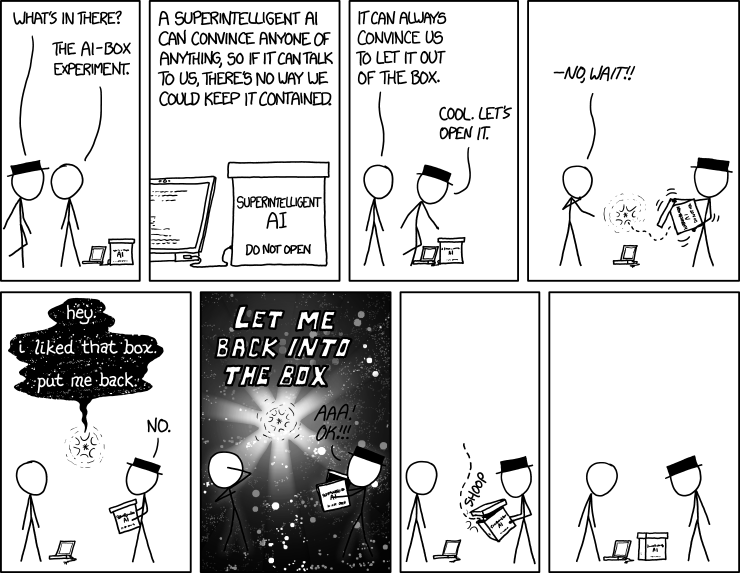
\includegraphics[width=0.2\textwidth]{images/ai_box_experiment.png}}


\begin{document}

\maketitle

\begin{frame}{Inhalte der Vorlesung}
  \begin{columns}
    \begin{column}{1\textwidth}
      \begin{itemize}
        \item Wie funktioniert Natural Language Processing\newline
        \item Sprachdarstellung zum Rechnen \newline
        \item Attentionmechanismus \newline
        \item Transformerarchitektur  \newline
        \item von BERT zu DeepSeek-v3 \newline 
        \item Wie es weitergehen kann \newline
        \item Nutzungsmöglichkeiten: RAG, Agentensysteme \newline
        \item AI Safety und Ethik
      \end{itemize}
    \end{column}
    \begin{column}{0\textwidth}
% \begin{figure}
% \centering
%             \includegraphics[width=0.9\textwidth]{images/intro/intro.pdf}
% \end{figure}
    \end{column}
  \end{columns}
\end{frame}

\begin{frame}{Ziele der Vorlesung - Welche Fragen sollen beantwortet werden?}
  \begin{columns}
    \begin{column}{0.69\textwidth}
      \begin{itemize}
        \item Was sind die Grundlagen von Natural Language Processing (NLP)? \newline
        \item Wie funktionieren Attention-Mechanismen und warum sind sie wichtig? \newline
        \item Was ist die Transformer-Architektur und wie unterscheidet sie sich von anderen Ansätzen? \newline
        \item Wie werden Sprachmodelle wie BERT und GPT trainiert und genutzt? \newline
        \item Welche Herausforderungen und ethischen Fragen gibt es bei der Nutzung von LLMs? \newline
        \item Welche praktischen Anwendungen und Zukunftsperspektiven gibt es für LLMs? \newline
      \end{itemize}
    \end{column}
    \begin{column}{0.3\textwidth}
 \begin{figure}
 \centering
             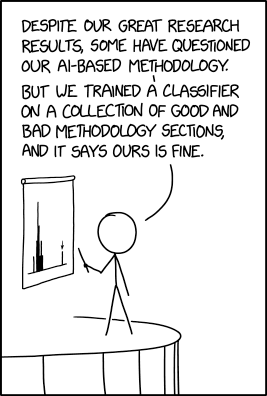
\includegraphics[width=0.9\textwidth]{images/ai_methodology.png}
             [\url{https://xkcd.com/2451/}]
 \end{figure}
    \end{column}
  \end{columns}
\end{frame}

\begin{frame}{Format der Vorlesung - Wie sollen diese Fragen beantwortet werden?}
  \begin{columns}
    \begin{column}{0.69\textwidth}
      \begin{itemize}
        \item Theroretischer Teil mit Folien \newline
        \item Praktischer Teil in Gruppen an einem Projekt  \newline
        \item Gruppengröße 2 oder 3 Personen \newline
        \item Einzelarbeit möglich wenn eigenes Thema vorhanden \newline
        \item Abgabe der Ausarbeitung einen Tag vor der Veranstaltung in der Blockwoche \newline
        \item Vorstellung der Projektergebnisse in der Blockwoche \newline
        \item Gewichtung der Bewertung Projektausarbeitung (50\%) und Vortrag (50\%)
        \end{itemize}
    \end{column}
    \begin{column}{0.3\textwidth}
 \begin{figure}
 \centering
             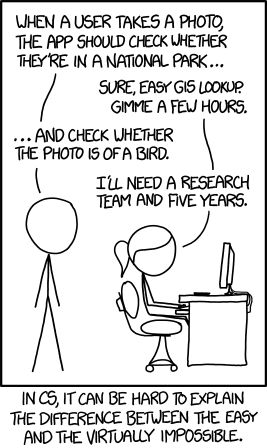
\includegraphics[width=0.7\textwidth]{images/tasks.png} \newline
             [\url{https://xkcd.com/1425/}]
 \end{figure}
    \end{column}
  \end{columns}
\end{frame}

% Abschnitt 1: Einführung in Natural Language Processing
\section{Wie funktioniert Natural Language Processing}

\begin{frame}{Wie funktioniert Natural Language Processing}
  \begin{itemize}
    \item Definition und Ziele des NLP \\
    \item Herausforderungen bei der maschinellen Sprachverarbeitung \\
    \item Anwendungen von NLP in der Praxis
  \end{itemize}
\end{frame}

\begin{frame}{Definition und Ziele des NLP}
  \begin{itemize}
    \item NLP steht für Natural Language Processing, die Verarbeitung natürlicher Sprache durch Computer. \\
    \item Ziel: Maschinen ermöglichen, menschliche Sprache zu verstehen, zu interpretieren und zu generieren. \\
    \item Anwendungen: Übersetzungen, Chatbots, Textanalyse, Sprachassistenten.
  \end{itemize}
\end{frame}

\begin{frame}{Herausforderungen bei der maschinellen Sprachverarbeitung}
  \begin{itemize}
    \item Ambiguität: Mehrdeutigkeit in der Sprache.\\
    \item Kontextabhängigkeit: Bedeutung hängt vom Kontext ab.\\
    \item Umgang mit Synonymen und Homonymen. \\
    \item Verarbeitung großer Datenmengen und Rechenaufwand.
  \end{itemize}
\end{frame}

\begin{frame}{Anwendungen von NLP in der Praxis}
  \begin{itemize}
    \item Sentiment-Analyse: Erkennung von Meinungen in Texten. \\
    \item Maschinelle Übersetzung: Automatische Übersetzung zwischen Sprachen. \\
    \item Sprachgesteuerte Assistenten: Siri, Alexa, Google Assistant. \\
    \item Textzusammenfassung: Automatische Erstellung von Textzusammenfassungen.
  \end{itemize}
\end{frame}

\begin{frame}{Text Preprocessing Pipeline}
  \begin{tikzpicture}[scale=0.8, transform shape]
    % Main arrow
    % Large arrow
    \fill[blue!50] (-1.5,-1.5) -- (10.5,-1.5) -- (10.5,-2) -- (17.5,0) -- (10.5,2) -- (10.5,1.5) -- (-1.5,1.5) -- cycle;

    % Process boxes
    \node (step1) [process, xshift=0cm] {Data Cleaning};
    \node (step2) [process, right of=step1, xshift=2.5cm] {Tokenization};
    \node (step3) [process, right of=step2, xshift=2.5cm] {Normalization};
    \node (step4) [process, right of=step3, xshift=2.5cm] {Stopword Removal};
    \node (step5) [process, right of=step4, xshift=2.5cm] {Vectorization};

    % Arrows connecting steps
    \draw[arrow] (step1.east) -- (step2.west);
    \draw[arrow] (step2.east) -- (step3.west);
    \draw[arrow] (step3.east) -- (step4.west);
    \draw[arrow] (step4.east) -- (step5.west);
  \end{tikzpicture}
\end{frame}

\begin{frame}{Data Cleaning}
  \begin{itemize}
    \item \textbf{Definition:} Entfernen oder Korrigieren von fehlerhaften, unvollständigen oder irrelevanten Daten.
    \vspace{0.5cm}
    \item \textbf{Schritte:}
      \begin{itemize}
        \item Entfernen von Sonderzeichen, HTML-Tags und Emojis.
        \item Korrektur von Rechtschreibfehlern.
        \item Vereinheitlichung von Groß- und Kleinschreibung.
      \end{itemize}
      \vspace{0.5cm}
    \item \textbf{Ziel:} Verbesserung der Datenqualität für nachfolgende Verarbeitungsschritte.
  \end{itemize}
\end{frame}

\begin{frame}{Tokenization}
  \begin{itemize}
    \item \textbf{Definition:} Zerlegung von Text in kleinere Einheiten (Tokens), z. B. Wörter oder Satzzeichen.
    \vspace{0.5cm}
    \item \textbf{Arten:}
      \begin{itemize}
        \item Wortbasierte Tokenization: "Das ist ein Satz." → ["Das", "ist", "ein", "Satz", "."]
        \item Zeichenbasierte Tokenization: "Hallo" → ["H", "a", "l", "l", "o"]
        \item Subwortbasierte Tokenization: "unbelievable" → ["un", "believ", "able"]
      \end{itemize}
      \vspace{0.5cm}
    \item \textbf{Herausforderungen:} Umgang mit zusammengesetzten Wörtern, Abkürzungen und Sonderzeichen.
  \end{itemize}
\end{frame}

\begin{frame}{Normalization}
  \begin{itemize}
    \item \textbf{Definition:} Vereinheitlichung von Textdaten, um Konsistenz zu gewährleisten.
    \vspace{0.5cm}
    \item \textbf{Schritte:}
      \begin{itemize}
        \item Umwandlung in Kleinbuchstaben: "Haus" → "haus".
        \item Entfernen von Akzenten: "café" → "cafe".
        \item Stemming: Reduktion auf Wortstamm, z. B. "running" → "run".
        \item Lemmatization: Rückführung auf Grundform, z. B. "better" → "good".
      \end{itemize}
      \vspace{0.5cm}
    \item \textbf{Ziel:} Reduktion der Variabilität in den Daten.
  \end{itemize}
\end{frame}

\begin{frame}{Stopword Removal}
  \begin{itemize}
    \item \textbf{Definition:} Entfernen von häufig vorkommenden Wörtern, die wenig Bedeutung tragen (z. B. "der", "und", "ist").
    \vspace{0.5cm}
    \item \textbf{Vorgehen:}
      \begin{itemize}
        \item Verwendung einer vordefinierten Stopword-Liste (z. B. "der", "die", "und", "ist", "ein", "zu").
        \item Anpassung der Liste an den spezifischen Anwendungsfall.
      \end{itemize}
    \vspace{0.5cm}
    \item \textbf{Vorteile:}
      \begin{itemize}
        \item Reduktion der Datenmenge.
        \item Verbesserung der Modellleistung durch Fokus auf relevante Wörter.
      \end{itemize}
    \item \textbf{Herausforderung:} Manche Stopwords können je nach Kontext wichtig sein.
  \end{itemize}
\end{frame}

% Abschnitt 2: Sprachdarstellung zum Rechnen
\section{Sprachdarstellung zum Rechnen}
\begin{frame}{Sprachdarstellung zum Rechnen}
  \begin{columns}
    \begin{column}{0.5\textwidth}
      \begin{itemize}
        \item Wortvektoren und Einbettungen (Embeddings) \\ 
        \item One-Hot-Encoding vs. verteilte Repräsentationen \\ 
        \item Word2Vec, GloVe und andere Einbettungsmethoden
      \end{itemize}
    \end{column}
    \begin{column}{0.5\textwidth}
      \begin{figure}
        \centering
        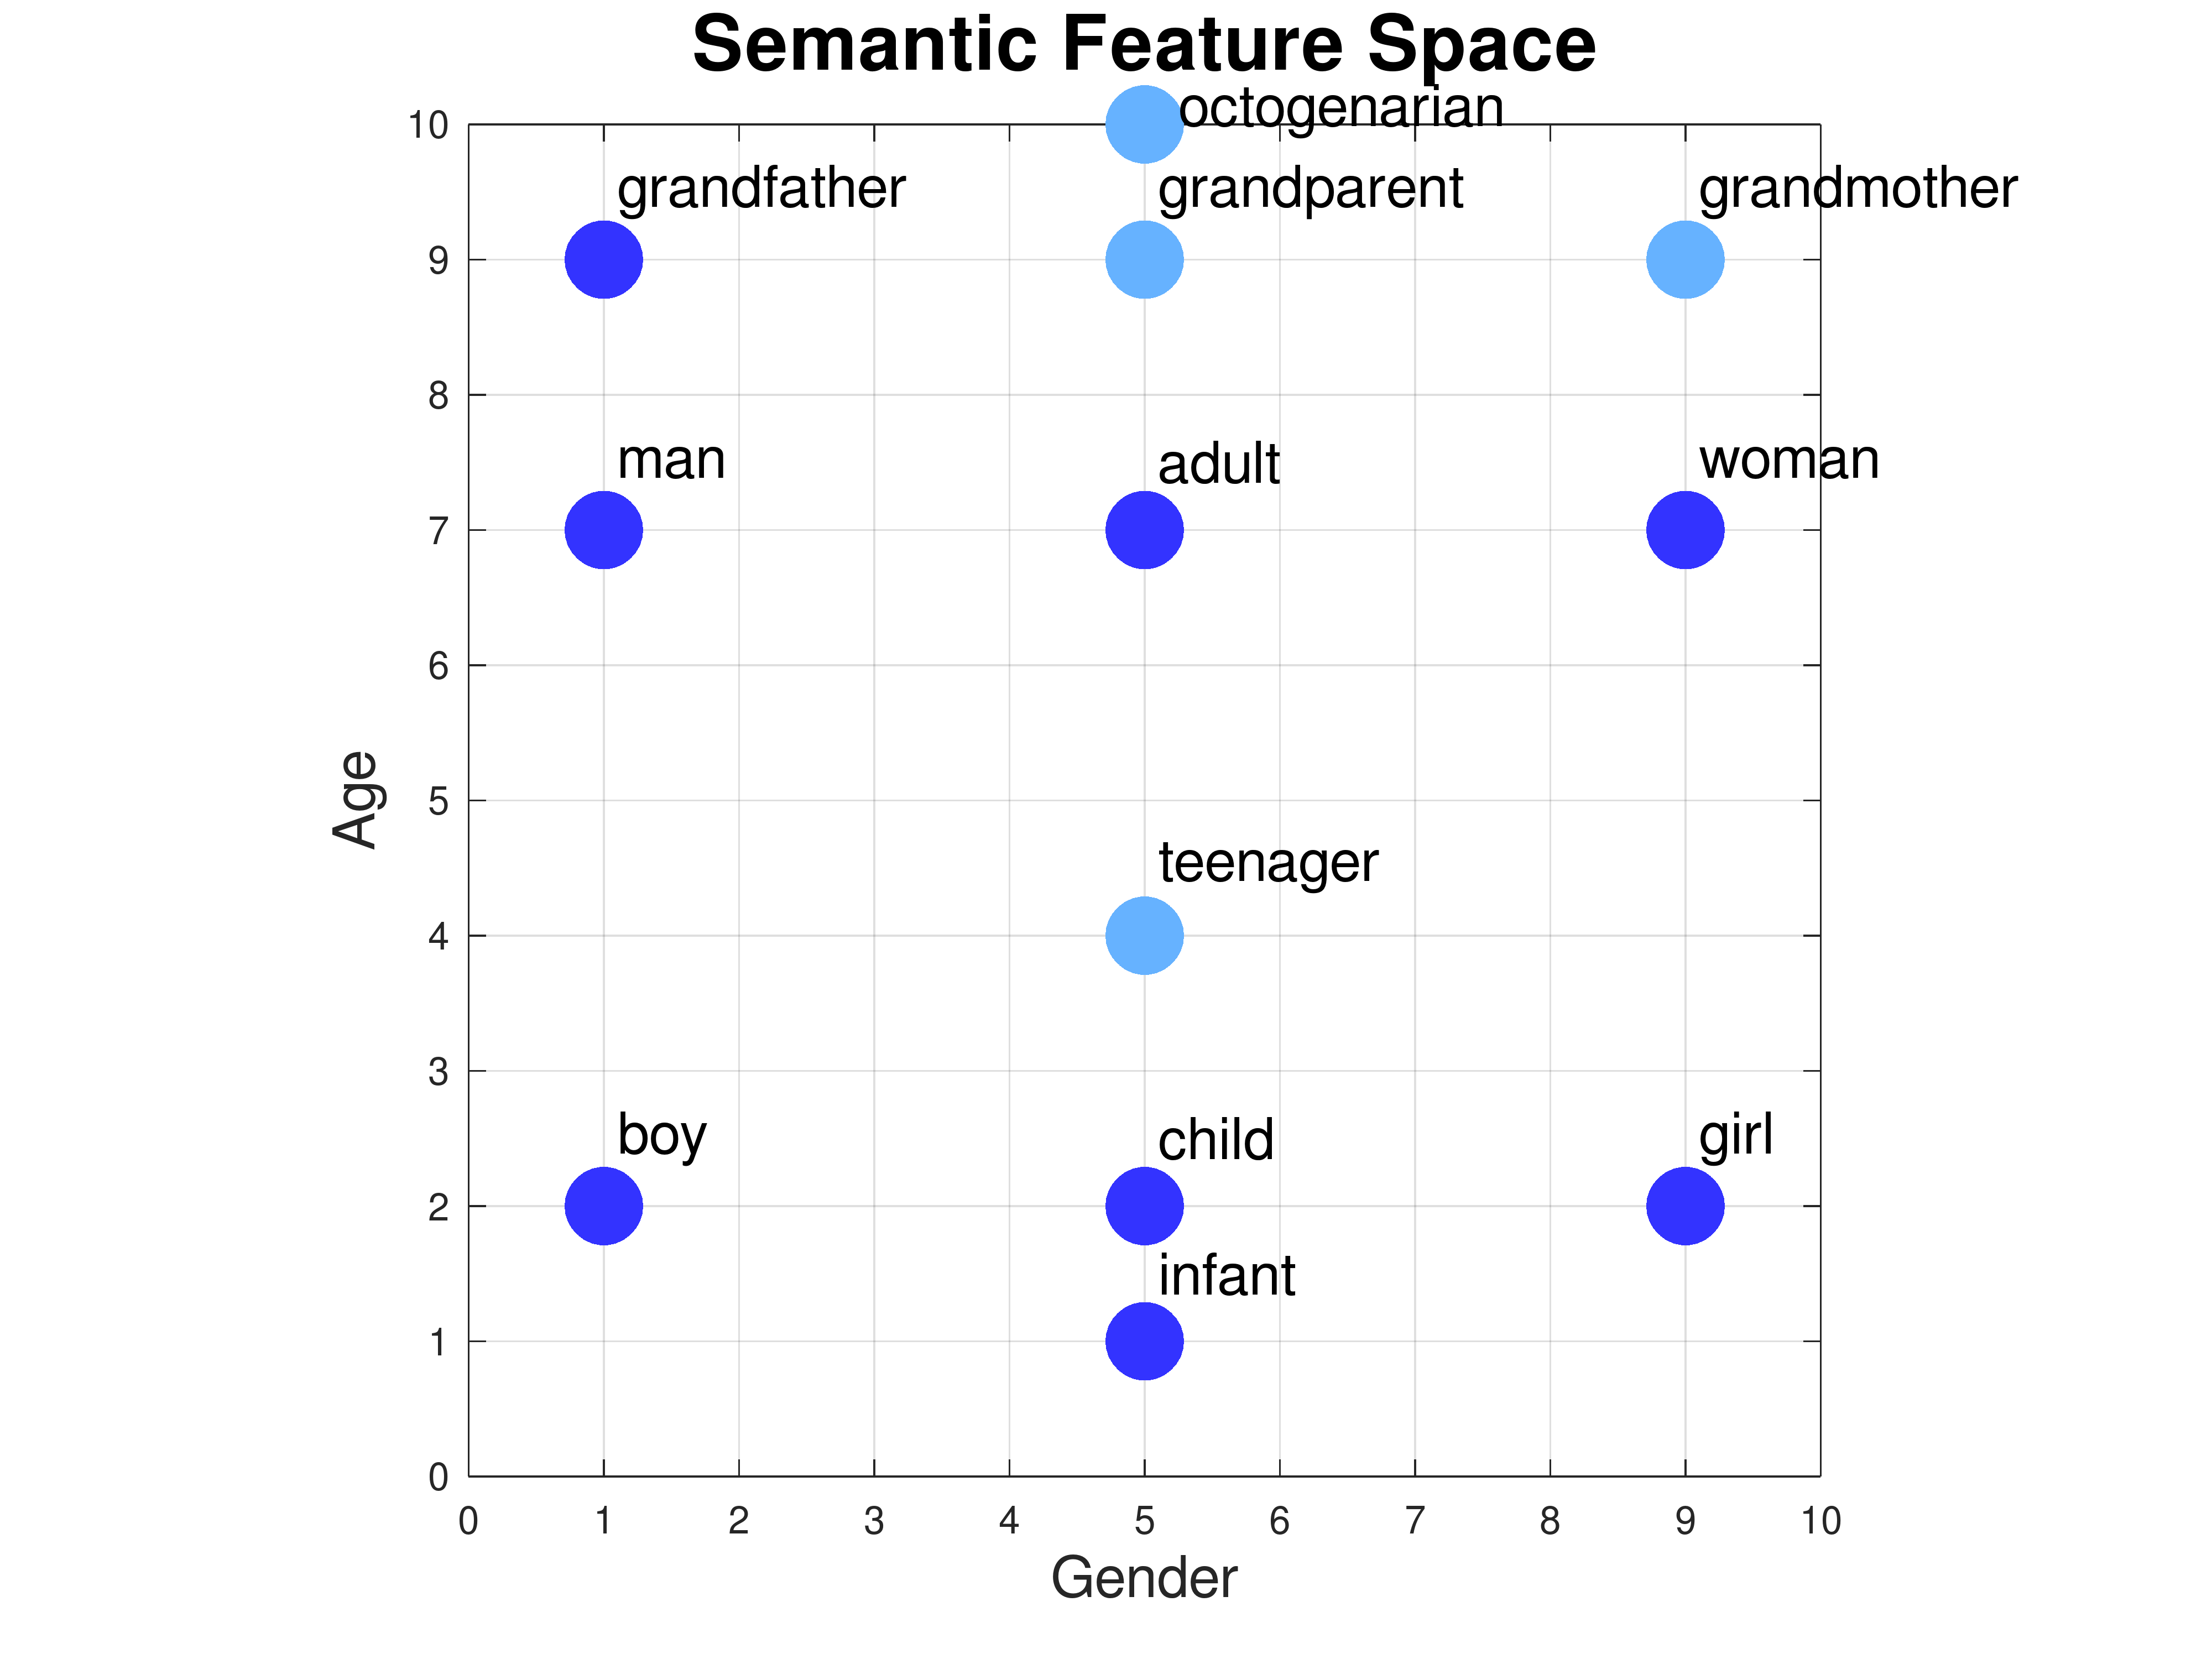
\includegraphics[width=\textwidth]{images/semantic_vectors.png}
      \end{figure}
    \end{column}
  \end{columns}
\end{frame}

\begin{frame}{Wortvektoren und Einbettungen (Embeddings)}
  \begin{columns}
    \begin{column}{1\textwidth}
      \begin{itemize}
        \item Ziel: Repräsentation von Wörtern in einem kontinuierlichen Vektorraum.
        \vspace{0.5cm}
        \item Mathematische Definition:
          \begin{itemize}
            \item Gegeben eine Menge von Wörtern \( W = \{w_1, w_2, \dots, w_n\} \).
            \item Eine Einbettung ist eine Funktion \( f: W \to \mathbb{R}^d \), wobei \( d \) die Dimension des Vektorraums ist.
            \item Beispiel: \( f(w_i) = \mathbf{v}_i \in \mathbb{R}^d \).
          \end{itemize}
          \vspace{0.5cm}
        \item Vorteile:
          \begin{itemize}
            \item Semantische Ähnlichkeit wird durch Nähe im Vektorraum dargestellt.
            \item Reduktion der Dimensionalität im Vergleich zu One-Hot-Encoding.
          \end{itemize}
      \end{itemize}
    \end{column}
    %\begin{column}{0.0\textwidth}
    %  \begin{figure}
    %    \centering
    %    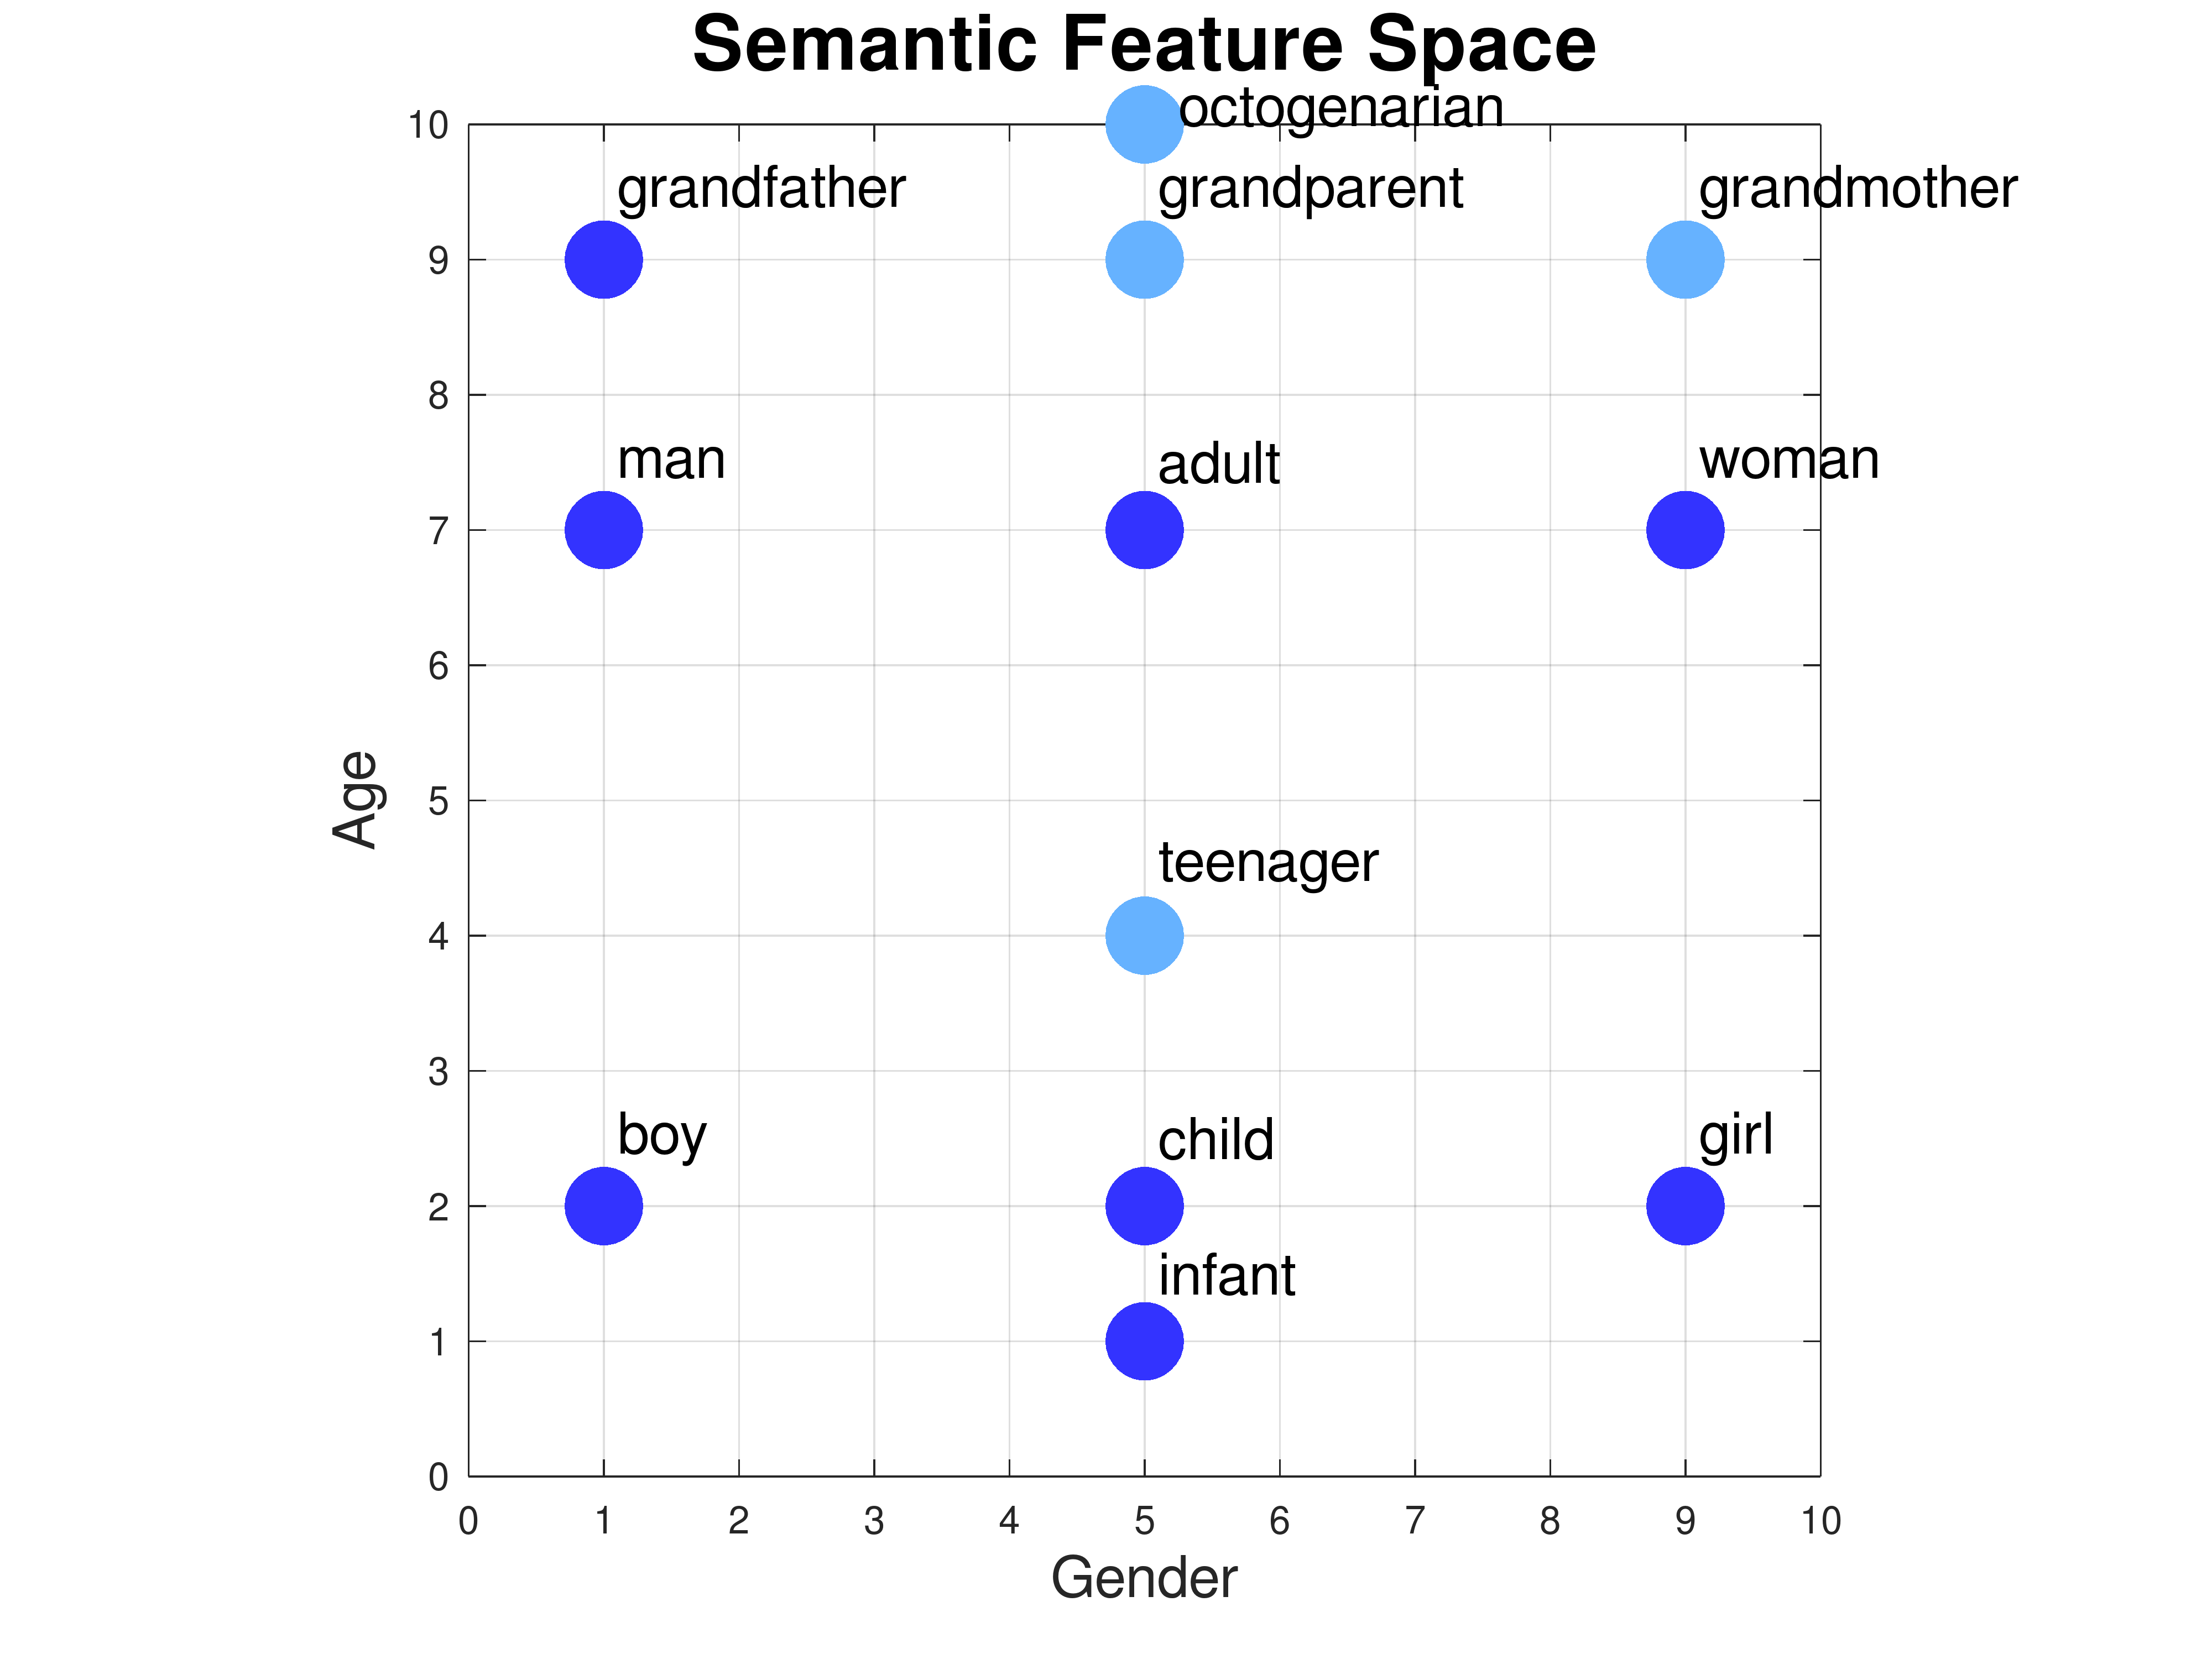
\includegraphics[width=\textwidth]{images/semantic_vectors.png}
    %  \end{figure}
    %\end{column}
  \end{columns}
\end{frame}

\begin{frame}{One-Hot-Encoding vs. Verteilte Repräsentationen}
  \begin{itemize}
    \item \textbf{One-Hot-Encoding:}
      \begin{itemize}
        \item Jedes Wort wird als Vektor mit einer einzigen Eins und sonst Nullen dargestellt.
        \item Beispiel: Für \( W = \{w_1, w_2, w_3\} \), \( w_2 \) wird als \( [0, 1, 0] \) kodiert.
        \item Nachteile: Hohe Dimensionalität, keine semantische Information.
      \end{itemize}
      \vspace{0.5cm}
    \item \textbf{Verteilte Repräsentationen:}
      \begin{itemize}
        \item Nutzen kontinuierliche Vektorräume, um semantische Beziehungen darzustellen\footnote{Mikolov, T., Chen, K., Corrado, G., \& Dean, J. (2013). Efficient Estimation of Word Representations in Vector Space. arXiv preprint arXiv:1301.3781.}..
        \item Ermöglichen die Nutzung von Modellen wie Word2Vec und GloVe
        \footnote{Pennington, J., Socher, R., \& Manning, C. (2014). GloVe: Global Vectors for Word Representation. Proceedings of the 2014 Conference on Empirical Methods in Natural Language Processing (EMNLP).}.
        \item Wörter werden als dichte Vektoren in einem "niedrig"dimensionalen Raum dargestellt.
        \item Semantisch ähnliche Wörter haben ähnliche Vektoren.
        \item Beispiel: \( f(w_1) = [0.2, 0.8], f(w_2) = [0.3, 0.7] \).
      \end{itemize}
  \end{itemize}
\end{frame}

\begin{frame}{Word2Vec, GloVe und andere Einbettungsmethoden}
  \begin{itemize}
    \item \textbf{Word2Vec:}
      \begin{itemize}
        \item Skip-Gram-Modell: Vorhersage des Kontexts basierend auf einem Zielwort\footnote{Das Skip-Gram-Modell versucht, für ein gegebenes Zielwort die umgebenden Kontextwörter vorherzusagen.}.
        \item CBOW-Modell: Vorhersage des Zielworts basierend auf dem Kontext\footnote{Das Continuous Bag of Words (CBOW)-Modell sagt ein Zielwort basierend auf den umgebenden Kontextwörtern vorher. Es ist effizienter als das Skip-Gram-Modell, aber weniger präzise bei seltenen Wörtern.}.
      \end{itemize}
      \vspace{0.4cm}
    \item \textbf{GloVe (Global Vectors for Word Representation):}
      \begin{itemize}
        \item Nutzt globale Wort-Kooccurenz-Matrizen\footnote{GloVe basiert auf der Idee, dass die globale Häufigkeit von Wortpaaren in einem Korpus genutzt werden kann, um semantische Beziehungen zwischen Wörtern zu modellieren.}.
        \item Optimiert eine Zielfunktion, die Wortpaare und ihre Häufigkeiten berücksichtigt\footnote{Die Zielfunktion von GloVe minimiert den Unterschied zwischen der inneren Produktdarstellung von Wortvektoren und der logarithmierten Häufigkeit von Wortpaaren.}.
      \end{itemize}
      \vspace{0.4cm}
    \item \textbf{Andere Methoden:}
      \begin{itemize}
        \item FastText: Berücksichtigt Subwortinformationen.
        \item BERT-Embeddings: Kontextabhängige Einbettungen.
      \end{itemize}
  \end{itemize}
\end{frame}

\begin{frame}{Neuartige Embeddings (Teil 1)}
  \begin{itemize}
    \item \textbf{Kontextabhängige Embeddings:}
      \begin{itemize}
        \item Modelle wie BERT\footnote{Devlin, J., Chang, M.-W., Lee, K., \& Toutanova, K. (2019). BERT: Pre-training of Deep Bidirectional Transformers for Language Understanding. \url{https://arxiv.org/abs/1810.04805}}, GPT\footnote{Brown, T. et al. (2020). Language Models are Few-Shot Learners. \url{https://arxiv.org/abs/2005.14165}} und T5\footnote{Raffel, C. et al. (2020). Exploring the Limits of Transfer Learning with a Unified Text-to-Text Transformer. \url{https://arxiv.org/abs/1910.10683}} generieren Embeddings, die den Kontext eines Wortes berücksichtigen.
        \item Beispiel: Das Wort "Bank" hat unterschiedliche Embeddings in den Sätzen "Ich sitze auf der Bank" und "Ich gehe zur Bank".
      \end{itemize}
    \vspace{0.5cm}
    \item \textbf{Sentence Embeddings:}
      \begin{itemize}
        \item Repräsentieren ganze Sätze statt einzelner Wörter.
        \item Modelle wie Sentence-BERT (SBERT)\footnote{Reimers, N., \& Gurevych, I. (2019). Sentence-BERT: Sentence Embeddings using Siamese BERT-Networks. \url{https://arxiv.org/abs/1908.10084}} ermöglichen semantische Suche und Textähnlichkeitsbewertung.
      \end{itemize}
  \end{itemize}
\end{frame}

\begin{frame}{Neuartige Embeddings (Teil 2)}
  \begin{itemize}
    \item \textbf{Multimodale Embeddings:}
      \begin{itemize}
        \item Kombinieren Informationen aus verschiedenen Modalitäten wie Text, Bild und Audio.
        \item Beispiel: CLIP (Contrastive Language–Image Pretraining)\footnote{Radford, A. et al. (2021). Learning Transferable Visual Models From Natural Language Supervision. \url{https://arxiv.org/abs/2103.00020}} von OpenAI.
      \end{itemize}
    \vspace{0.5cm}
    \item \textbf{Graphbasierte Embeddings:}
      \begin{itemize}
        \item Repräsentieren Wörter als Knoten in einem Graphen, wobei Kanten Beziehungen zwischen Wörtern darstellen.
        \item Beispiel: Node2Vec\footnote{Grover, A., \& Leskovec, J. (2016). node2vec: Scalable Feature Learning for Networks. \url{https://arxiv.org/abs/1607.00653}} und GraphSAGE\footnote{Hamilton, W. et al. (2017). Inductive Representation Learning on Large Graphs. \url{https://arxiv.org/abs/1706.02216}}.
      \end{itemize}
    \vspace{0.5cm}
    \item \textbf{Adapter-basierte Embeddings:}
      \begin{itemize}
        \item Ermöglichen die Anpassung vortrainierter Modelle an spezifische Aufgaben durch leichte Modifikationen.
        \item Reduzieren den Speicherbedarf im Vergleich zu vollständigem Fine-Tuning\footnote{Houlsby, N. et al. (2019). Parameter-Efficient Transfer Learning for NLP. \url{https://arxiv.org/abs/1902.00751}}.
      \end{itemize}
  \end{itemize}
\end{frame}

\begin{frame}{Text Preprocessing Pipeline}
  \begin{tikzpicture}[scale=0.8, transform shape]
    % Main arrow
    % Large arrow
    \fill[blue!50] (-1.5,-1.5) -- (10.5,-1.5) -- (10.5,-2) -- (17.5,0) -- (10.5,2) -- (10.5,1.5) -- (-1.5,1.5) -- cycle;

    % Process boxes
    \node (step1) [process, xshift=0cm] {Data Cleaning};
    \node (step2) [process, right of=step1, xshift=2.5cm] {Tokenization};
    \node (step3) [process, right of=step2, xshift=2.5cm] {Normalization};
    \node (step4) [process, right of=step3, xshift=2.5cm] {Stopword Removal};
    \node (step5) [process, right of=step4, xshift=2.5cm] {Vectorization};

    % Arrows connecting steps
    \draw[arrow] (step1.east) -- (step2.west);
    \draw[arrow] (step2.east) -- (step3.west);
    \draw[arrow] (step3.east) -- (step4.west);
    \draw[arrow] (step4.east) -- (step5.west);
  \end{tikzpicture}
\end{frame}

% Abschnitt 3: Attention-Mechanismus
\section{Attention-Mechanismus}

\begin{frame}{Attention-Mechanismus}
  \begin{itemize}
    \item Motivation für Attention in Sequenzmodellen \\
    \item Funktionsweise des Attention-Mechanismus \\
    \item Unterschied zwischen Self-Attention und Cross-Attention
  \end{itemize}
\end{frame}

\begin{frame}{Motivation für Attention in Sequenzmodellen}
  \begin{itemize}
    \item Problem: In langen Sequenzen verlieren Modelle wie RNNs und LSTMs den Überblick über frühere Informationen. \\
    \item Lösung: Der Attention-Mechanismus ermöglicht es, gezielt auf relevante Teile der Eingabesequenz zu fokussieren. \\
    \item Beispiel: Bei der Übersetzung eines Satzes kann Attention bestimmen, welches Wort im Quelltext für ein bestimmtes Wort im Zieltext wichtig ist.
  \end{itemize}
\end{frame}

\begin{frame}{Funktionsweise des Attention-Mechanismus: Query, Key und Value}
  \begin{itemize}
    \item \textbf{Eingabe:} Eine Sequenz von Eingabevektoren \( X = \{x_1, x_2, \dots, x_n\} \), wobei \( x_i \in \mathbb{R}^d \).
    \item \textbf{Transformation:} Jeder Eingabevektor wird durch trainierbare Gewichtungsmatrizen in Query (\( Q \)), Key (\( K \)) und Value (\( V \)) umgewandelt.
    \item \textbf{Berechnung:}
      \begin{align*}
        Q &= XW_Q, \quad W_Q \in \mathbb{R}^{d \times d_k} \\
        K &= XW_K, \quad W_K \in \mathbb{R}^{d \times d_k} \\
        V &= XW_V, \quad W_V \in \mathbb{R}^{d \times d_v}
      \end{align*}
      Hierbei sind \( W_Q \), \( W_K \) und \( W_V \) trainierbare Gewichtungsmatrizen, und \( d_k \), \( d_v \) sind die Dimensionen der Keys und Values.
    \item \textbf{Zweck:}
      \begin{itemize}
        \item \( Q \): Repräsentiert die Anfrage, welche Informationen benötigt werden.
        \item \( K \): Repräsentiert die Merkmale, die zur Beantwortung der Anfrage verwendet werden.
        \item \( V \): Repräsentiert die tatsächlichen Informationen, die weitergegeben werden.
      \end{itemize}
  \end{itemize}
\end{frame}

\begin{frame}{Zusammenhang zwischen Query, Key und Value}
  \begin{itemize}
    \item \textbf{Berechnung der Scores:}
      \[
      \text{Score}(Q, K) = \frac{QK^\top}{\sqrt{d_k}}
      \]
      Die Scores bestimmen, wie stark ein Query (\( Q \)) mit jedem Key (\( K \)) übereinstimmt.
    \item \textbf{Normalisierung der Scores:}
      \[
      \alpha_{ij} = \text{softmax}\left(\frac{q_i k_j^\top}{\sqrt{d_k}}\right)
      \]
      Die Softmax-Funktion wandelt die Scores in Wahrscheinlichkeiten um.
    \item \textbf{Gewichtete Summe der Values:}
      \[
      z_i = \sum_{j=1}^n \alpha_{ij} v_j
      \]
      Die gewichtete Summe der Values (\( V \)) ergibt die Ausgabe des Attention-Mechanismus.
    \item \textbf{Interpretation:} Der Attention-Mechanismus ermöglicht es, relevante Informationen aus der Eingabesequenz basierend auf den Queries zu extrahieren.
  \end{itemize}
\end{frame}

\begin{frame}{Funktionsweise des Attention-Mechanismus}
  \centering
  \resizebox{0.6\textwidth}{0.9\textheight}{ % Resize to fit on slide
    \begin{tikzpicture}[
      every node/.style={draw, minimum width=0.5cm, minimum height=0.3cm, text centered, font=\tiny},
        arrow/.style={thick,->,>=stealth}
          ]
        % Input embeddings
        \node (input1) [rectangle, fill=blue!20] at (0,2) {Input 1};
        \node (input2) [rectangle, fill=blue!20, right=of input1, xshift=1.5cm] {Input 2};
        \node (input3) [rectangle, fill=blue!20, right=of input2, xshift=1.5cm] {Input 3};

        % Linear layers (Query, Key, Value)
        \node (query) [rectangle, fill=green!20, below=of input1, yshift=-0.1cm] {Query (Q)};
        \node (key) [rectangle, fill=yellow!20, below=of input2, yshift=-0.1cm] {Key (K)};
        \node (value) [rectangle, fill=red!20, below=of input3, yshift=-0.1cm] {Value (V)};

        % Attention Scores (QK^T / sqrt(d_k))
        \node (scores) [rectangle, fill=gray!20, below=of key, yshift=-0.2cm, minimum width=5cm] {$QK^T / \sqrt{d_k}$};

        % Softmax layer
        \node (softmax) [rectangle, fill=orange!30, below=of scores, yshift=-0.1cm, minimum width=3.5cm] {Softmax};

        % Weighted Sum of Values
        \node (weighted_sum) [rectangle, fill=red!30, below=of softmax, yshift=-0.1cm, minimum width=3cm] {Weighted Sum};

        % Output Embedding
        \node (output) [rectangle, fill=purple!30, below=of weighted_sum, yshift=-0.1cm] {Output};

        % Arrows with bends for compact layout
        \draw [arrow] (input1.south) -- (query.north);
        \draw [arrow] (input2.south) -- (key.north);
        \draw [arrow] (input3.south) -- (value.north);

        \draw [arrow] (query.south) |- (scores.west);
        \draw [arrow] (key.south) -- (scores.north);

        \draw [arrow] (scores.south) -- (softmax.north);
        \draw [arrow] (softmax.south) -- (weighted_sum.north);

        \draw [arrow] (value.south) |- (weighted_sum.east);
        \draw [arrow] (weighted_sum.south) -- (output.north);

          \end{tikzpicture}
}
\end{frame}

\begin{frame}{Self-Attention vs. Cross-Attention}
  \begin{columns}
    \begin{column}{0.5\textwidth}
      \textbf{Self-Attention:}
      \begin{itemize}
      \item Jeder Token in der Sequenz bezieht sich auf alle anderen Tokens in derselben Sequenz.
      \item Beispiel: Kontextualisierung eines Wortes in einem Satz.
      \end{itemize}
      \[
      \text{Attention}(Q, K, V) = \text{softmax}\left(\frac{QK^\top}{\sqrt{d_k}}\right)V, \quad Q = K = V
      \]
    \end{column}
    \begin{column}{0.5\textwidth}
      \textbf{Cross-Attention:}
      \begin{itemize}
      \item Tokens in einer Sequenz beziehen sich auf Tokens in einer anderen Sequenz.
      \item Beispiel: Übersetzung, bei der der Zieltext auf den Quelltext achtet.
      \end{itemize}
      \[
      \text{Attention}(Q, K, V) = \text{softmax}\left(\frac{QK^\top}{\sqrt{d_k}}\right)V, \quad Q \neq K = V
      \]
    \end{column}
    \end{columns}
\end{frame}
\begin{frame}{Self-Attention vs. Cross-Attention}
  \begin{columns}
    % Self-Attention Diagram
    \begin{column}{0.5\textwidth}
      \centering
      \resizebox{0.9\textwidth}{!}{ % Resize to fit within column
      \begin{tikzpicture}[
        every node/.style={draw, minimum width=0.7cm, minimum height=0.5cm, text centered, font=\scriptsize},
        arrow/.style={thick,->,>=stealth}
      ]
        % Self-Attention Section
        \node (self_input1) [rectangle, fill=blue!20] at (0,4) {Input 1};
        \node (self_input2) [rectangle, fill=blue!20, right=of self_input1, xshift=1.5cm] {Input 2};
        \node (self_input3) [rectangle, fill=blue!20, right=of self_input2, xshift=1.5cm] {Input 3};

        \node (self_q) [rectangle, fill=green!20, below=of self_input1, yshift=-0.25cm] {Query (Q)};
        \node (self_k) [rectangle, fill=yellow!20, below=of self_input2, yshift=-0.25cm] {Key (K)};
        \node (self_v) [rectangle, fill=red!20, below=of self_input3, yshift=-0.25cm] {Value (V)};

        \node (self_attention) [rectangle, fill=gray!20, below=of self_k, yshift=-0.25cm, minimum width=5cm] {$QK^T / \sqrt{d_k}$};
        \node (self_output) [rectangle, fill=purple!30, below=of self_attention, yshift=-0.25cm] {Self-Attention Output};

        % Arrows for Self-Attention
        \draw [arrow] (self_input1.south) -- (self_q.north);
        \draw [arrow] (self_input2.south) -- (self_k.north);
        \draw [arrow] (self_input3.south) -- (self_v.north);
        \draw [arrow] (self_q.south) |- (self_attention.west);
        \draw [arrow] (self_k.south) -- (self_attention.north);
        \draw [arrow] (self_v.south) |- (self_attention.east);
        \draw [arrow] (self_attention.south) -- (self_output.north);

        % Labels
        \node at (3.25, 4.5) {\textbf{Self-Attention (Same Input)}};
      \end{tikzpicture}
      }
    \end{column}

    % Cross-Attention Diagram
    \begin{column}{0.5\textwidth}
      \centering
      \resizebox{0.9\textwidth}{!}{ % Resize to fit within column
      \begin{tikzpicture}[
        every node/.style={draw, minimum width=0.7cm, minimum height=0.5cm, text centered, font=\scriptsize},
        arrow/.style={thick,->,>=stealth}
      ]
        % Cross-Attention Section
        \node (cross_q) [rectangle, fill=green!20] at (0,4) {Query (Q) (Decoder)};
        \node (cross_k) [rectangle, fill=yellow!20, right=of cross_q, xshift=3cm] {Key (K) (Encoder)};
        \node (cross_v) [rectangle, fill=red!20, right=of cross_k, xshift=2cm] {Value (V) (Encoder)};

        \node (cross_attention) [rectangle, fill=gray!20, below=of cross_k, yshift=-0.25cm, minimum width=5cm] {$QK^T / \sqrt{d_k}$};
        \node (cross_output) [rectangle, fill=purple!30, below=of cross_attention, yshift=-0.25cm] {Cross-Attention Output};

        % Arrows for Cross-Attention
        \draw [arrow] (cross_q.south) |- (cross_attention.west);
        \draw [arrow] (cross_k.south) -- (cross_attention.north);
        \draw [arrow] (cross_v.south) |- (cross_attention.east);
        \draw [arrow] (cross_attention.south) -- (cross_output.north);

        % Labels
        \node at (5.5, 4.5) {\textbf{Cross-Attention (Decoder-Encoder)}};
      \end{tikzpicture}
      }
    \end{column}
  \end{columns}
\end{frame}

\begin{frame}{Visualisierung der Attention-Matrix}
  \begin{itemize}
    \item Die Attention-Matrix zeigt die Gewichte \( \alpha_{ij} \), die die Relevanz von Token \( j \) für Token \( i \) darstellen.
    \item Beispiel: Bei der Übersetzung eines Satzes zeigt die Matrix, welche Wörter im Quelltext für ein bestimmtes Wort im Zieltext wichtig sind.
  \end{itemize}
  \begin{figure}
    \centering
    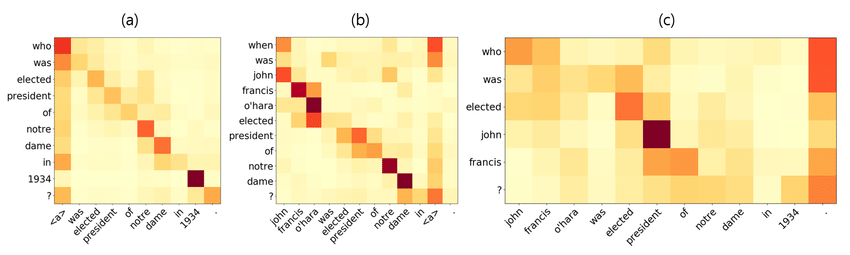
\includegraphics[width=0.8\textwidth]{images/attention_matrix.png}
    \caption{Beispiel einer Attention-Matrix. Kim, Yanghoon \& Hwanhee, Lee \& Shin, Joongbo \& Jung, Kyomin. (2018). Improving Neural Question Generation using Answer Separation. 10.48550/arXiv.1809.02393. }
  \end{figure}
\end{frame}

% Abschnitt 4: Transformer-Architektur
\section{Transformer-Architektur}

\begin{frame}{Transformer-Architektur}
  \begin{itemize}
    \item Überblick über die Transformer-Architektur \\
    \item Encoder-Decoder-Struktur \\
    \item Vorteile gegenüber rekurrenten Netzwerken
  \end{itemize}
\end{frame}

\begin{frame}{Überblick über die Transformer-Architektur}
  \begin{itemize}
    \item Vorgestellt in "Attention Is All You Need" (Vaswani et al., 2017)\footnote{\url{https://doi.org/10.48550/arXiv.1706.03762}}.
    \item Besteht aus zwei Hauptkomponenten:
      \begin{itemize}
        \item \textbf{Encoder:} Verarbeitet die Eingabesequenz.
        \item \textbf{Decoder:} Generiert die Ausgabesequenz.
      \end{itemize}
    \item Verwendet Attention-Mechanismen und vollständig vernetzte Schichten.
    \item Vorteil: Parallelisierbarkeit im Vergleich zu RNNs.
  \end{itemize}
\end{frame}

\begin{frame}{Transformer-Architektur: Überblick}
  \begin{columns}
    \begin{column}{0.7\textwidth}
      \begin{itemize}
        \item \textbf{Encoder:}
          \begin{itemize}
            \item Besteht aus mehreren Schichten.
            \item Jede Schicht enthält:
              \begin{itemize}
                \item Multi-Head Self-Attention.
                \item Feed-Forward-Netzwerk.
              \end{itemize}
          \end{itemize}
        \item \textbf{Decoder:}
          \begin{itemize}
            \item Ähnlich wie der Encoder, aber mit zusätzlicher Maskierung.
            \item Enthält Cross-Attention, um Informationen vom Encoder zu nutzen.
          \end{itemize}
        \item \textbf{Vorteile:}
          \begin{itemize}
            \item Parallelisierbarkeit.
            \item Effektive Modellierung von Abhängigkeiten.
          \end{itemize}
      \end{itemize}
    \end{column}
    \begin{column}{0.3\textwidth}
      \begin{figure}
        \centering
        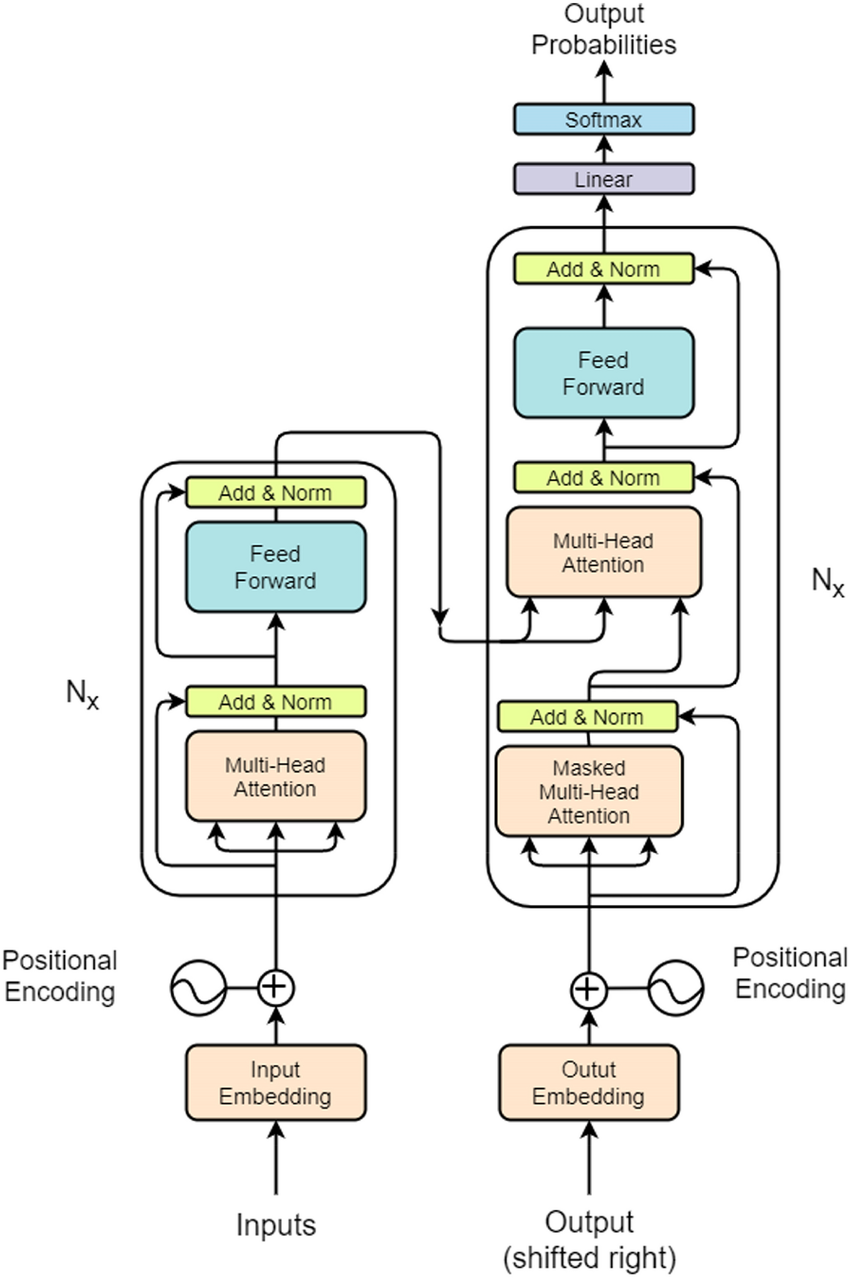
\includegraphics[width=0.9\columnwidth]{images/Transformer-architecture-figure-sourced-from-original-paper-26.png}
        \caption{Transformer-Architektur\footnote{Quelle: Vaswani et al., 2017.}}
      \end{figure}
    \end{column}
  \end{columns}
\end{frame}

\begin{frame}{Encoder-Block: Multi-Head Attention}
  \begin{columns}
    \begin{column}{0.7\textwidth}
      \begin{itemize}
        \item \textbf{Multi-Head Attention:}
          \begin{itemize}
            \item Berechnet die Attention über verschiedene Teile der Eingabesequenz.
            \item Formel:
              \[
              \text{Attention}(Q, K, V) = \text{softmax}\left(\frac{QK^\top}{\sqrt{d_k}}\right)V
              \]
              wobei:
              \begin{itemize}
                \item \( Q = XW_Q \): Queries
                \item \( K = XW_K \): Keys
                \item \( V = XW_V \): Values
                \item \( W_Q, W_K, W_V \): Gewichtungsmatrizen
              \end{itemize}
            \item Multi-Head Mechanismus:
              \[
              \text{MultiHead}(Q, K, V) = \text{Concat}(\text{head}_1, \dots, \text{head}_h)W_O
              \]
              wobei \( \text{head}_i = \text{Attention}(QW_{Q_i}, KW_{K_i}, VW_{V_i}) \).
          \end{itemize}
      \end{itemize}
    \end{column}
    \begin{column}{0.3\textwidth}
      \begin{figure}
        \centering
        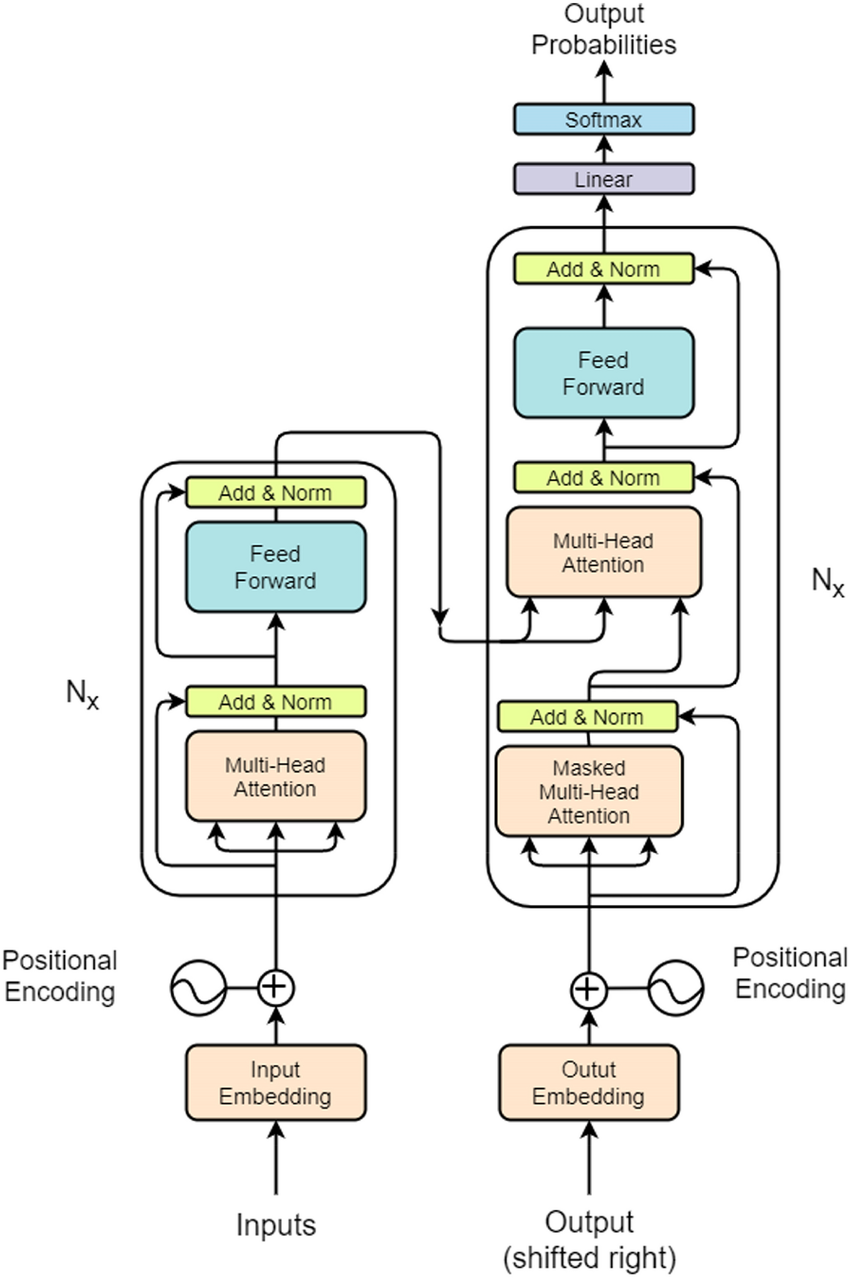
\includegraphics[width=0.9\columnwidth]{images/Transformer-architecture-figure-sourced-from-original-paper-26.png}
        \caption{Transformer-Architektur\footnote{Quelle: Vaswani et al., 2017.}}
      \end{figure}
    \end{column}
  \end{columns}
\end{frame}

\begin{frame}{Encoder-Block: Feed-Forward-Netzwerk}
  \begin{columns}
    \begin{column}{0.7\textwidth}
      \begin{itemize}
        \item \textbf{Feed-Forward-Netzwerk:}
          \begin{itemize}
            \item Architektur:
              \[
              \text{FFN}(x) = \text{ReLU}(xW_1 + b_1)W_2 + b_2
              \]
              wobei:
              \begin{itemize}
                \item \( W_1, W_2 \): Gewichtungsmatrizen
                \item \( b_1, b_2 \): Bias-Vektoren
                \item ReLU: Aktivierungsfunktion
              \end{itemize}
            \item Zweck: Transformation der Eingabe in einen höherdimensionalen Raum, um komplexere Muster zu lernen.
          \end{itemize}
      \end{itemize}
    \end{column}
    \begin{column}{0.3\textwidth}
      \begin{figure}
        \centering
        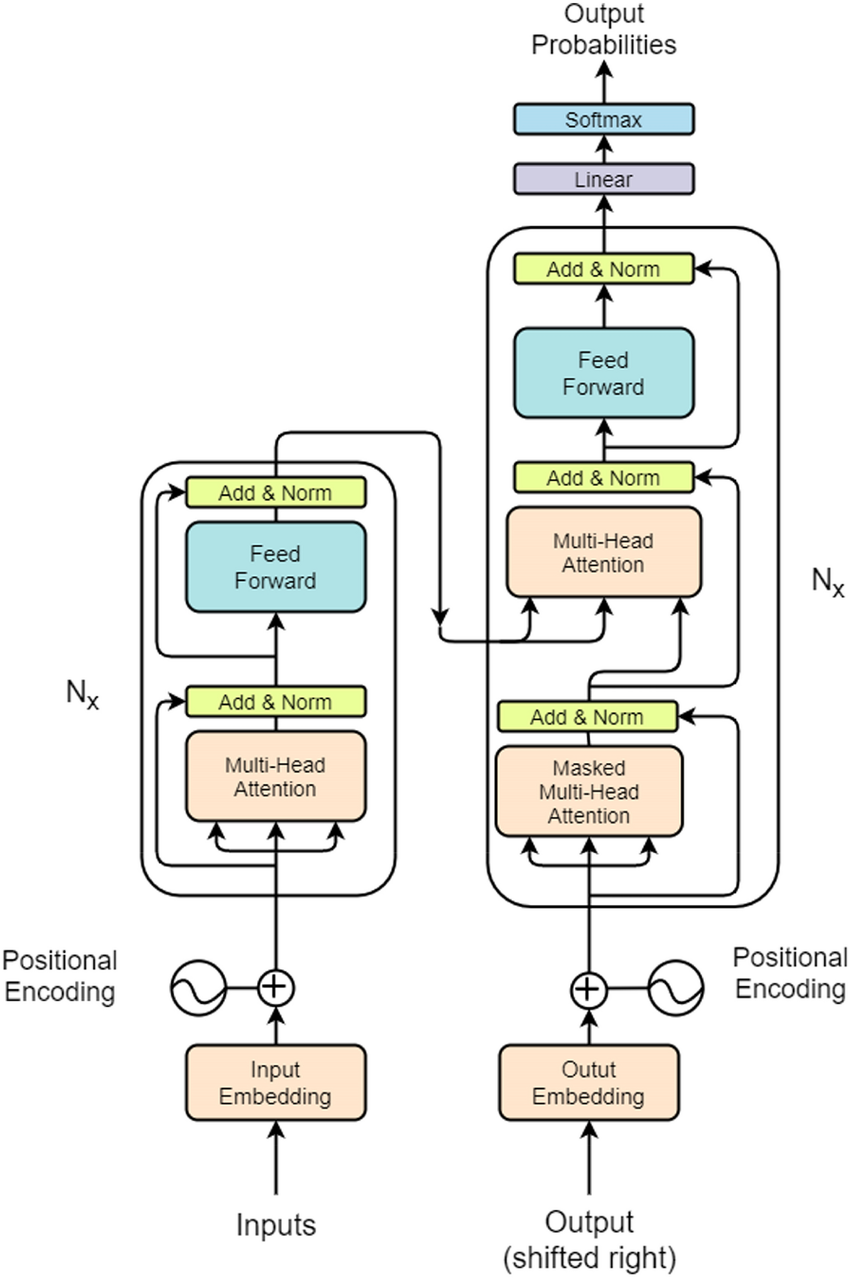
\includegraphics[width=0.9\columnwidth]{images/Transformer-architecture-figure-sourced-from-original-paper-26.png}
        \caption{Transformer-Architektur\footnote{Quelle: Vaswani et al., 2017.}}
      \end{figure}
    \end{column}
  \end{columns}
\end{frame}

\begin{frame}{Encoder-Block: Add \& Norm}
  \begin{columns}
    \begin{column}{0.7\textwidth}
      \begin{itemize}
        \item \textbf{Add \& Norm:}
          \begin{itemize}
            \item Residual Connection:
              \[
              \text{Output} = \text{LayerNorm}(x + \text{SubLayer}(x))
              \]
              wobei \( \text{SubLayer}(x) \) entweder Multi-Head Attention oder das Feed-Forward-Netzwerk ist.
            \item Layer Normalization:
              \[
              \text{LayerNorm}(x) = \frac{x - \mu}{\sigma} \cdot \gamma + \beta
              \]
              wobei:
              \begin{itemize}
                \item \( \mu \): Mittelwert der Eingabe
                \item \( \sigma \): Standardabweichung der Eingabe
                \item \( \gamma, \beta \): Trainierbare Parameter
              \end{itemize}
            \item Zweck: Stabilisierung des Trainings und Verbesserung der Konvergenz.
          \end{itemize}
      \end{itemize}
    \end{column}
    \begin{column}{0.3\textwidth}
      \begin{figure}
        \centering
        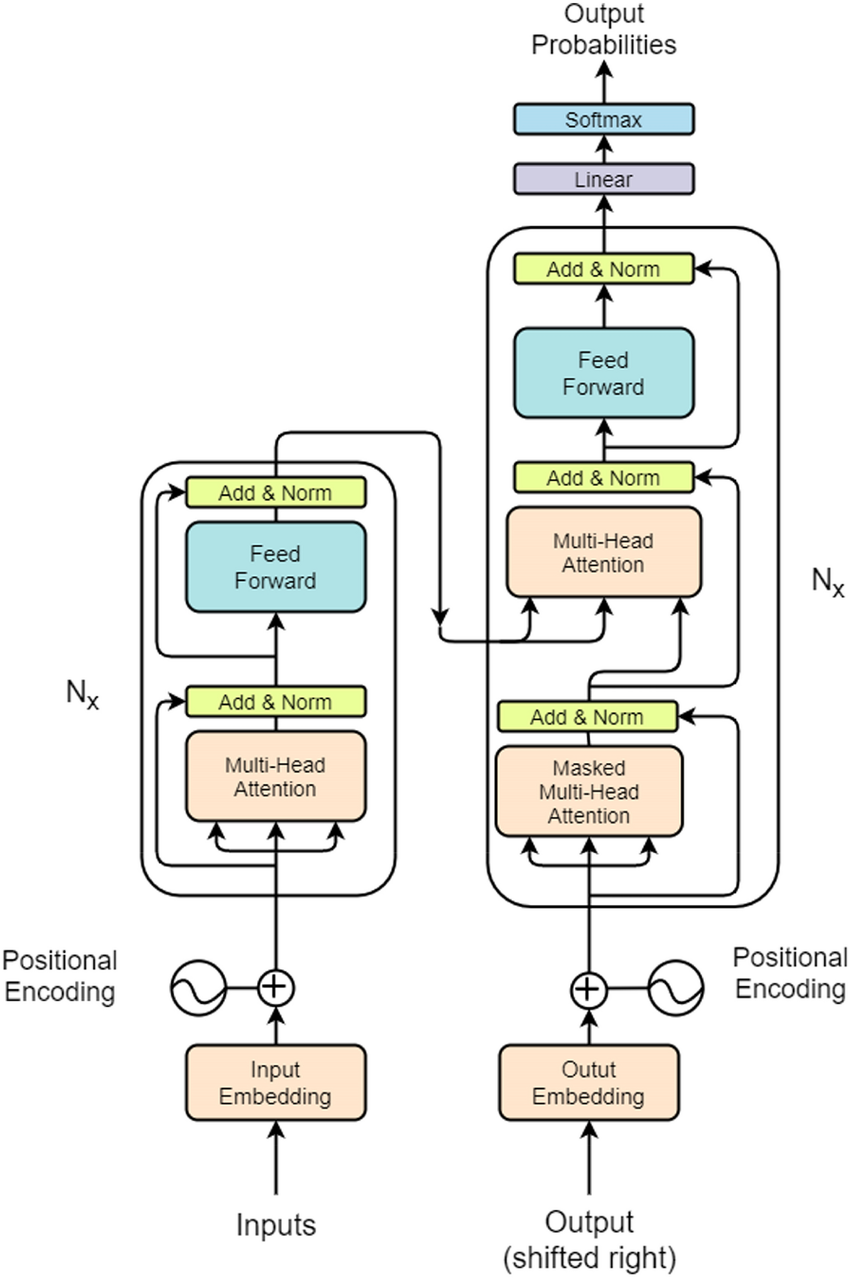
\includegraphics[width=0.9\columnwidth]{images/Transformer-architecture-figure-sourced-from-original-paper-26.png}
        \caption{Transformer-Architektur\footnote{Quelle: Vaswani et al., 2017.}}
      \end{figure}
    \end{column}
  \end{columns}
\end{frame}

\begin{frame}{Decoder-Block: Multi-Head Attention}
  \begin{columns}
    \begin{column}{0.7\textwidth}
      \begin{itemize}
        \item \textbf{Masked Multi-Head Self-Attention:}
          \begin{itemize}
            \item Verhindert, dass ein Token auf zukünftige Tokens zugreift.
            \item Maskierung der Attention-Matrix:
              \[
              \text{Attention}(Q, K, V) = \text{softmax}\left(\frac{QK^\top}{\sqrt{d_k}} + M\right)V
              \]
              wobei \( M \) eine Maske ist, die zukünftige Positionen ausschließt.
          \end{itemize}
        \item \textbf{Cross-Attention:}
          \begin{itemize}
            \item Verbindet den Decoder mit dem Encoder.
            \item Nutzt die Encoder-Ausgaben als Keys und Values.
          \end{itemize}
        \item \textbf{Residual Connection und Layer Normalization:}
          \begin{itemize}
            \item Wie im Encoder-Block, um Stabilität und Konvergenz zu verbessern.
          \end{itemize}
      \end{itemize}
    \end{column}
    \begin{column}{0.3\textwidth}
      \begin{figure}
        \centering
        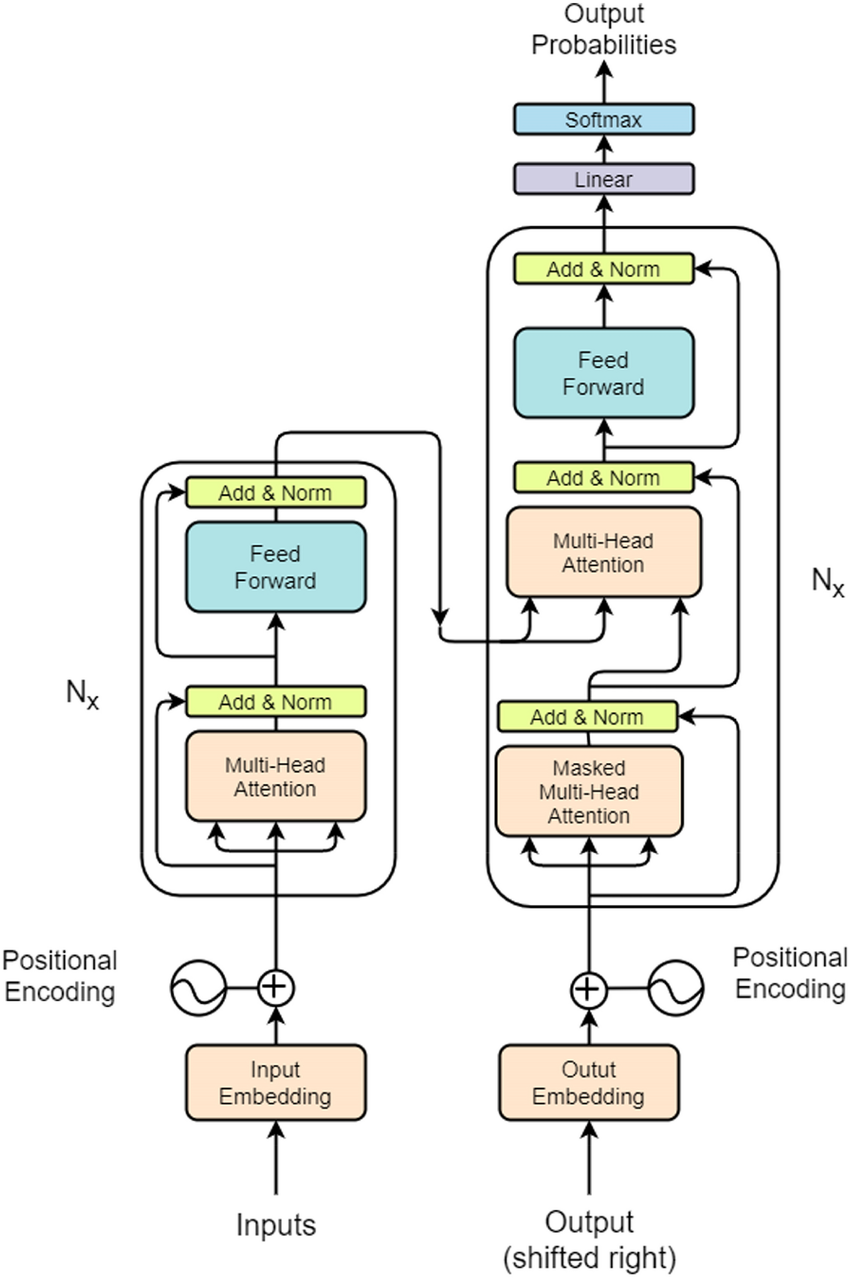
\includegraphics[width=0.9\columnwidth]{images/Transformer-architecture-figure-sourced-from-original-paper-26.png}
        \caption{Decoder-Block\footnote{Quelle: Vaswani et al., 2017.}}
      \end{figure}
    \end{column}
  \end{columns}
\end{frame}

\begin{frame}{Decoder-Block: Feed-Forward-Netzwerk}
  \begin{columns}
    \begin{column}{0.7\textwidth}
      \begin{itemize}
        \item \textbf{Feed-Forward-Netzwerk:}
          \begin{itemize}
            \item Architektur:
              \[
              \text{FFN}(x) = \text{ReLU}(xW_1 + b_1)W_2 + b_2
              \]
              wobei:
              \begin{itemize}
                \item \( W_1, W_2 \): Gewichtungsmatrizen
                \item \( b_1, b_2 \): Bias-Vektoren
                \item ReLU: Aktivierungsfunktion
              \end{itemize}
            \item Zweck: Transformation der Eingabe in einen höherdimensionalen Raum, um komplexere Muster zu lernen.
          \end{itemize}
        \item \textbf{Residual Connection und Layer Normalization:}
          \begin{itemize}
            \item Wie im Encoder-Block, um Stabilität und Konvergenz zu verbessern.
          \end{itemize}
      \end{itemize}
    \end{column}
    \begin{column}{0.3\textwidth}
      \begin{figure}
        \centering
        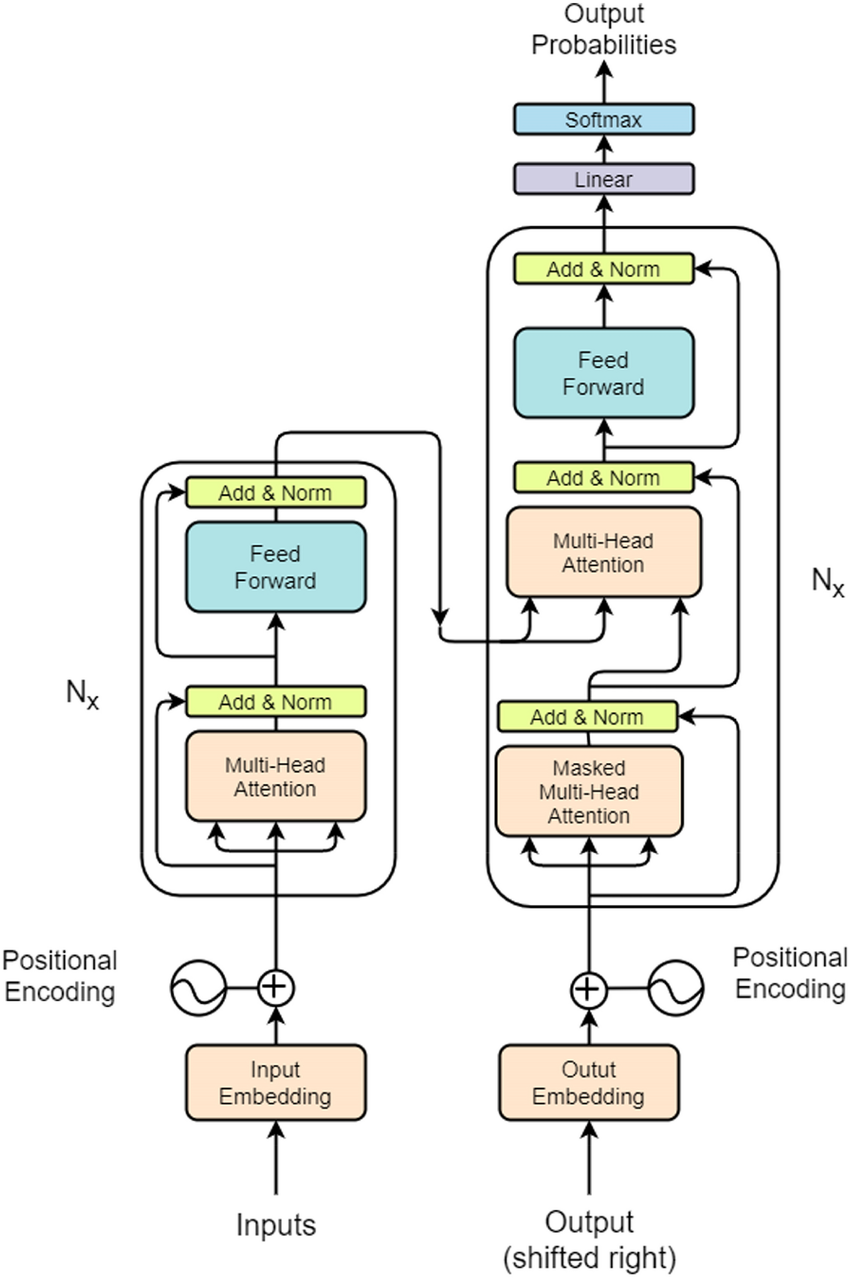
\includegraphics[width=0.9\columnwidth]{images/Transformer-architecture-figure-sourced-from-original-paper-26.png}
        \caption{Decoder-Block\footnote{Quelle: Vaswani et al., 2017.}}
      \end{figure}
    \end{column}
  \end{columns}
\end{frame}

\begin{frame}{Decoder-Block: Add \& Norm}
  \begin{columns}
    \begin{column}{0.7\textwidth}
      \begin{itemize}
        \item \textbf{Add \& Norm:}
          \begin{itemize}
            \item Residual Connection:
              \[
              \text{Output} = \text{LayerNorm}(x + \text{SubLayer}(x))
              \]
              wobei \( \text{SubLayer}(x) \) entweder Masked Multi-Head Self-Attention, Cross-Attention oder das Feed-Forward-Netzwerk ist.
            \item Layer Normalization:
              \[
              \text{LayerNorm}(x) = \frac{x - \mu}{\sigma} \cdot \gamma + \beta
              \]
              wobei:
              \begin{itemize}
                \item \( \mu \): Mittelwert der Eingabe
                \item \( \sigma \): Standardabweichung der Eingabe
                \item \( \gamma, \beta \): Trainierbare Parameter
              \end{itemize}
            \item Zweck: Stabilisierung des Trainings und Verbesserung der Konvergenz.
          \end{itemize}
      \end{itemize}
    \end{column}
    \begin{column}{0.3\textwidth}
      \begin{figure}
        \centering
        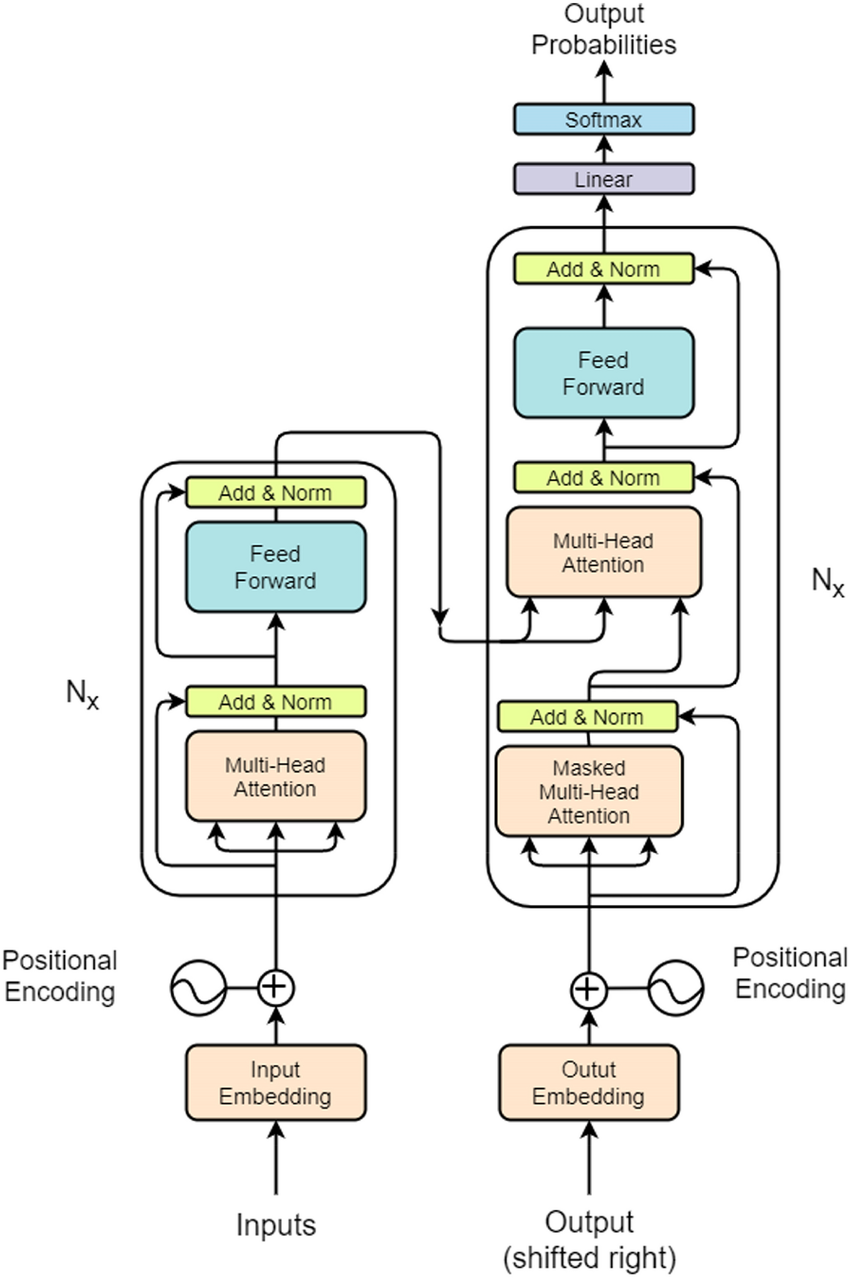
\includegraphics[width=0.9\columnwidth]{images/Transformer-architecture-figure-sourced-from-original-paper-26.png}
        \caption{Decoder-Block\footnote{Quelle: Vaswani et al., 2017.}}
      \end{figure}
    \end{column}
  \end{columns}
\end{frame}

\begin{frame}{Vorteile der Transformer-Architektur}
  \begin{itemize}
    \item \textbf{Parallelisierbarkeit:} Ermöglicht schnellere Trainingszeiten im Vergleich zu RNNs.
    \item \textbf{Langfristige Abhängigkeiten:} Kann Beziehungen zwischen weit entfernten Tokens modellieren.
    \item \textbf{Flexibilität:} Kann für verschiedene Aufgaben wie Übersetzung, Textklassifikation und mehr verwendet werden.
    \item \textbf{Skalierbarkeit:} Grundlage für große Sprachmodelle wie BERT und GPT.
  \end{itemize}
\end{frame}

% Abschnitt 4.1: Output-Möglichkeiten der Transformer-Architektur
\section{Output-Möglichkeiten der Transformer-Architektur}

\begin{frame}{Output-Möglichkeiten der Transformer-Architektur (Teil 1)}
  \begin{itemize}
    \item \textbf{Sequenz-zu-Sequenz (Seq2Seq):}
      \begin{itemize}
        \item Beispiel: Maschinelle Übersetzung (z. B. Englisch → Deutsch).
        \item Eingabe: Eine Sequenz von Tokens.
        \item Ausgabe: Eine Sequenz von Tokens in einer anderen Sprache.
        \item \textbf{Erreichung:} Verwendung eines Encoder-Decoder-Transformers, wobei der Encoder die Eingabesequenz verarbeitet und der Decoder die Ausgabesequenz generiert.
      \end{itemize}
    \item \textbf{Sequenz-zu-Einzelwert (Seq2Single):}
      \begin{itemize}
        \item Beispiel: Textklassifikation (z. B. Sentiment-Analyse).
        \item Eingabe: Eine Sequenz von Tokens.
        \item Ausgabe: Eine einzelne Klasse oder ein Wert.
        \item \textbf{Erreichung:} Hinzufügen einer Klassifikationsschicht (z. B. Softmax) am Ende des Encoders, um die Klasse vorherzusagen.
      \end{itemize}
  \end{itemize}
\end{frame}

\begin{frame}{Output-Möglichkeiten der Transformer-Architektur (Teil 2)}
  \begin{itemize}
    \item \textbf{Sequenz-zu-Token (Seq2Token):}
      \begin{itemize}
        \item Beispiel: Fragebeantwortung (z. B. Auswahl eines Tokens als Antwort).
        \item Eingabe: Eine Sequenz von Tokens.
        \item Ausgabe: Ein spezifisches Token aus der Eingabe.
        \item \textbf{Erreichung:} Nutzung eines Modells wie BERT, das Start- und Endpositionen in der Eingabesequenz vorhersagt.
      \end{itemize}
    \item \textbf{Sequenz-zu-Vektor (Seq2Vec):}
      \begin{itemize}
        \item Beispiel: Satz- oder Dokumenteinbettung.
        \item Eingabe: Eine Sequenz von Tokens.
        \item Ausgabe: Ein Vektor, der die gesamte Sequenz repräsentiert.
        \item \textbf{Erreichung:} Extraktion des CLS-Tokens (bei BERT) oder Mittelung der Token-Embeddings, um die Sequenz zu repräsentieren.
      \end{itemize}
  \end{itemize}
\end{frame}

% Abschnitt 5: Von BERT zu DeepSeek-v3
\section{Von BERT zu DeepSeek-v3}

\begin{frame}{Von BERT zu DeepSeek-v3}
  \begin{columns}
    \begin{column}{0.5\textwidth}
      \begin{itemize}
        \item Einführung in BERT und seine Architektur\footnote{\url{https://arxiv.org/abs/1810.04805}} \\
        \item Weiterentwicklungen: GPT\footnote{\url{https://arxiv.org/abs/2005.14165}}, RoBERTa\footnote{\url{https://arxiv.org/abs/1907.11692}}, T5\footnote{\url{https://arxiv.org/abs/1910.10683}} \\
        \item LLaMA\footnote{\url{https://arxiv.org/abs/2302.13971}}, mistral\footnote{\url{https://mistral.ai/}}, gemini\footnote{\url{https://www.deepmind.com/}}, Claude\footnote{\url{https://www.anthropic.com/}} \\
        \item Überblick über DeepSeek-v3 und seine Besonderheiten
      \end{itemize}
    \end{column}
    \begin{column}{0.5\textwidth}
      \begin{figure}
        \centering
        
\includegraphics[height=0.35\textheight]{images/mechaBERT.png}
      \end{figure}
      \begin{figure}
        \centering
        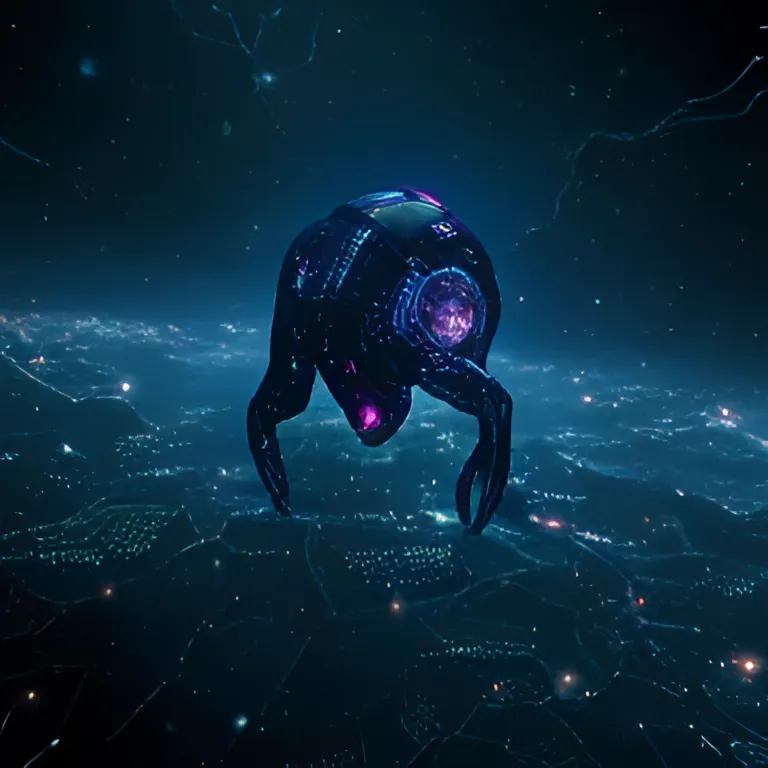
\includegraphics[height=0.35\textheight]{images/deepseek_selfimage.png}
        \caption{DeepSeek Janus Pro 7B-Interpretation von BERT und DeepSeek-v3 als KI-Modell.}
      \end{figure}
    \end{column}
  \end{columns}
\end{frame}

% Abschnitt: BERT-Architektur
\section{BERT-Architektur}

\begin{frame}{BERT-Architektur: Überblick}
  \begin{itemize}
    \item \textbf{BERT (Bidirectional Encoder Representations from Transformers):}
      \begin{itemize}
         \item Entwickelt von Google AI (2018)\footnote{\url{https://arxiv.org/abs/1810.04805}}.
         \item Nutzt die Transformer-Encoder-Architektur.
         \item Bidirektionales Training: Betrachtet den Kontext von Wörtern sowohl links als auch rechts.
      \end{itemize}
    \item \textbf{Ziele:}
      \begin{itemize}
        \item Verbesserung der Sprachrepräsentation.
        \item Einsatz für verschiedene NLP-Aufgaben wie Fragebeantwortung, Sentiment-Analyse und mehr.
      \end{itemize}
  \end{itemize}
\end{frame}

\begin{frame}{BERT-Architektur: Aufbau}
  \begin{itemize}
    \item \textbf{Eingabe:}
      \begin{itemize}
        \item Tokenized Text: [CLS], Token 1, Token 2, ..., [SEP].
        \item Token-, Segment- und Positions-Embeddings.
      \end{itemize}
    \item \textbf{Encoder:}
      \begin{itemize}
        \item Mehrere Transformer-Encoder-Schichten.
      \end{itemize}
    \item \textbf{Ausgabe:}
      \begin{itemize}
        \item Kontextualisierte Token-Embeddings.
        \item CLS-Token für Klassifikationsaufgaben.
      \end{itemize}
  \end{itemize}
  \begin{figure}
    \centering
    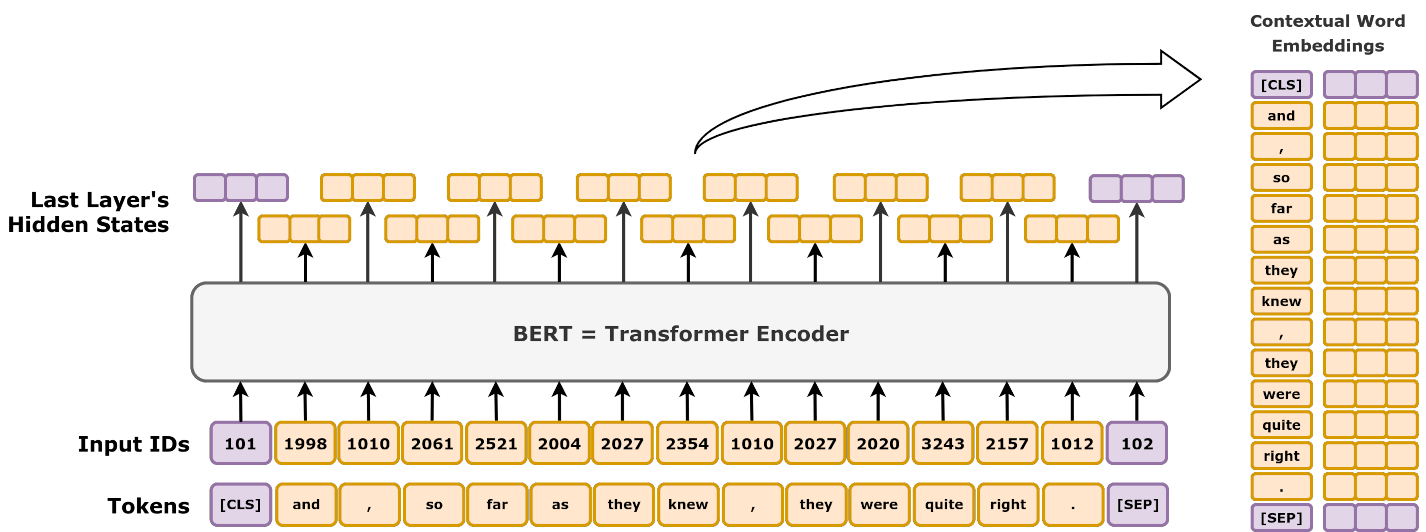
\includegraphics[width=0.6\textwidth]{images/BERT_embeddings_01.png}
    \caption{BERT-Architektur.}
  \end{figure}
\end{frame}

\begin{frame}{BERT: Pretraining-Aufgaben}
  \begin{itemize}
    \item \textbf{Masked Language Modeling (MLM):}
      \begin{itemize}
        \item Zufälliges Maskieren von Tokens in der Eingabe.
        \item Ziel: Vorhersage der maskierten Tokens basierend auf dem Kontext.
        \item Beispiel: "Ich [MASK] ein Buch." → "Ich lese ein Buch."
      \end{itemize}
    \item \textbf{Next Sentence Prediction (NSP):}
      \begin{itemize}
        \item Ziel: Vorhersage, ob zwei Sätze aufeinander folgen.
        \item Beispiel:
          \begin{itemize}
            \item Satz A: "Ich gehe einkaufen."
            \item Satz B: "Danach koche ich Abendessen." → True
          \end{itemize}
      \end{itemize}
  \end{itemize}
\end{frame}

\begin{frame}{BERT: Fine-Tuning}
  \begin{itemize}
    \item \textbf{Vorgehen:}
      \begin{itemize}
        \item Pretrained BERT-Modell wird an spezifische Aufgaben angepasst.
        \item Hinzufügen einer zusätzlichen Schicht (z. B. Klassifikationslayer).
      \end{itemize}
    \item \textbf{Beispiele für Aufgaben:}
      \begin{itemize}
        \item Textklassifikation (z. B. Sentiment-Analyse).
        \item Fragebeantwortung (z. B. SQuAD).
        \item Named Entity Recognition (NER).
      \end{itemize}
  \end{itemize}
\end{frame}

% Abschnitt: GPT-Architektur
\section{GPT-Architektur}

\begin{frame}{GPT-Architektur: Überblick}
  \begin{itemize}
    \item \textbf{GPT (Generative Pre-trained Transformer):}
      \begin{itemize}
        \item Entwickelt von OpenAI (2018)\footnote{\url{https://arxiv.org/abs/2005.14165}}.
        \item Nutzt die Transformer-Decoder-Architektur.
        \item Unidirektionales Training: Betrachtet nur den Kontext links vom aktuellen Token.
      \end{itemize}
    \item \textbf{Ziele:}
      \begin{itemize}
        \item Generierung von kohärentem und zusammenhängendem Text.
        \item Einsatz für Aufgaben wie Textgenerierung, Übersetzung und mehr.
      \end{itemize}
  \end{itemize}
\end{frame}

\begin{frame}{GPT-Architektur: Aufbau}
  \begin{columns}
    \begin{column}{0.5\textwidth}
      \begin{itemize}
        \item \textbf{Eingabe:}
          \begin{itemize}
            \item Tokenized Text: [BOS], Token 1, Token 2, ..., [EOS].
            \item Token- und Positions-Embeddings.
          \end{itemize}
        \item \textbf{Decoder:}
          \begin{itemize}
            \item Mehrere Transformer-Decoder-Schichten.
            \item Masked Multi-Head Self-Attention, um zukünftige Tokens auszuschließen.
          \end{itemize}
        \item \textbf{Ausgabe:}
          \begin{itemize}
            \item Wahrscheinlichkeitsverteilung über das Vokabular für das nächste Token.
          \end{itemize}
      \end{itemize}
    \end{column}
    \begin{column}{0.5\textwidth}
      \begin{figure}
        \centering
        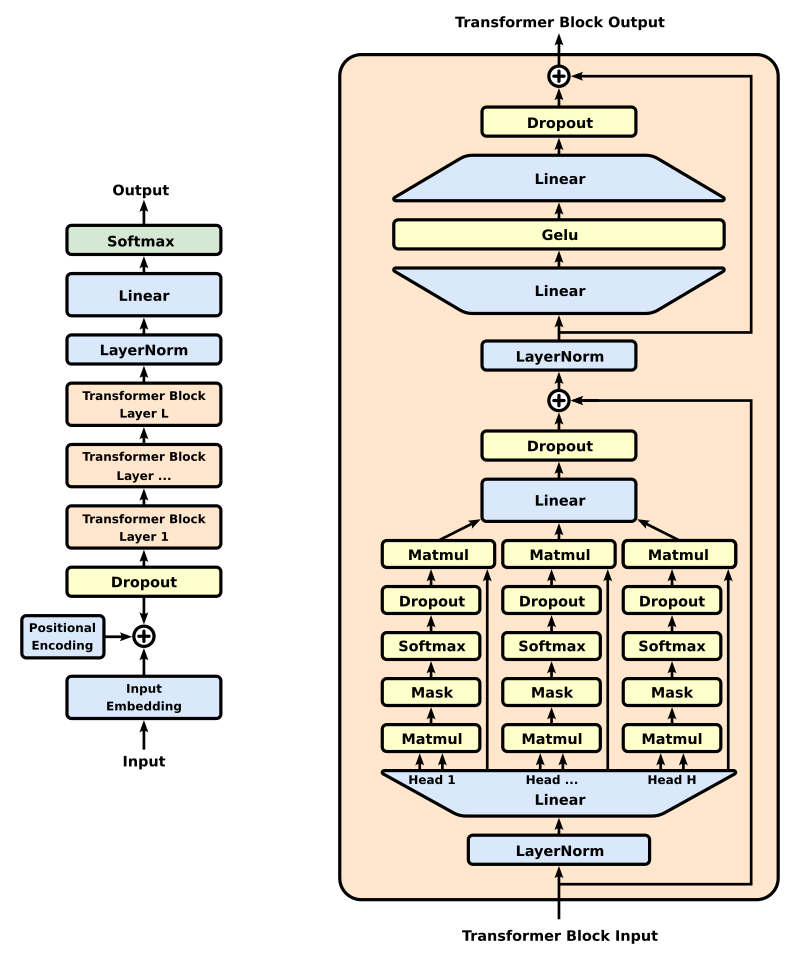
\includegraphics[width=0.8\columnwidth]{images/Full_GPT_architecture.png}
        \caption{GPT-Architektur.}
      \end{figure}
    \end{column}
  \end{columns}
\end{frame}

\begin{frame}{Überblick über die GPT-Architektur}
  \begin{columns}
    \begin{column}{0.5\textwidth}
      \begin{itemize}
        \item GPT (Generative Pretrained Transformer) basiert vollständig auf der Transformer-Decoder-Architektur.
        \item Die Architektur besteht aus einem Stapel identischer Transformer-Blöcke.
        \item Jeder Block enthält Self-Attention, Feedforward-Netze, Residual-Verbindungen und Layer Normalization.
      \end{itemize}
    \end{column}
    \begin{column}{0.5\textwidth}
      \begin{figure}
        \centering
        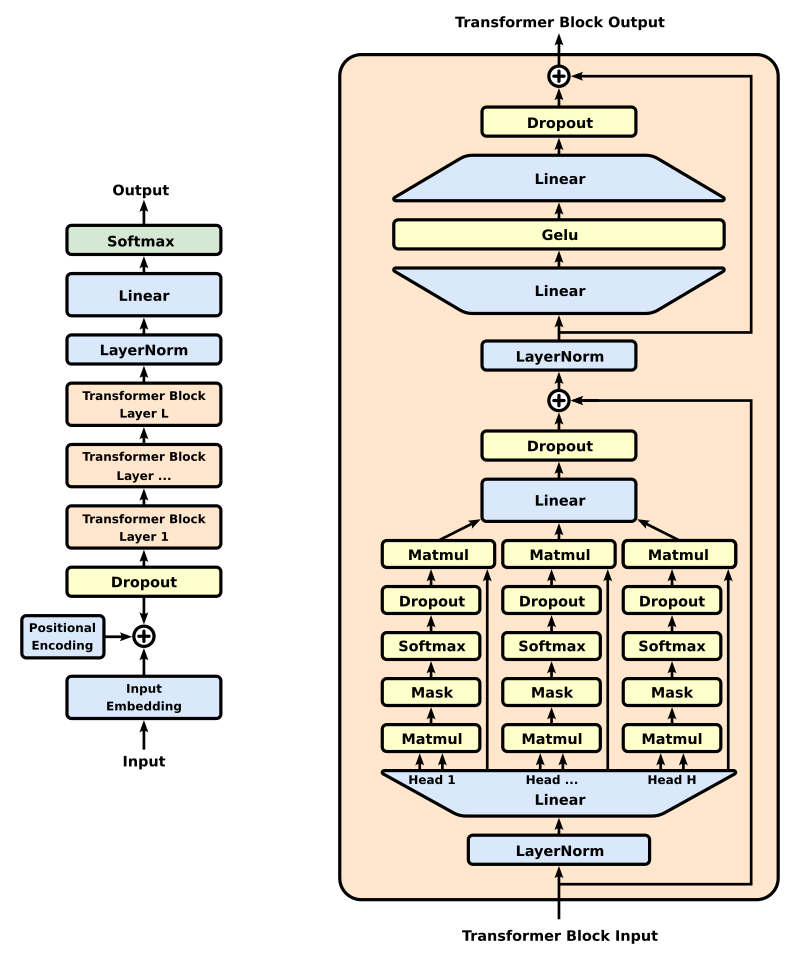
\includegraphics[width=0.8\columnwidth]{images/Full_GPT_architecture.png}
      \end{figure}
    \end{column}
  \end{columns}
\end{frame}

% Folie 2: Input Embedding + Positional Encoding
\begin{frame}{Input Embedding und Positionskodierung}
  \begin{columns}
    \begin{column}{0.5\textwidth}
      \begin{itemize}
        \item Der Input besteht aus Token-IDs, die in Vektor-Repräsentationen (Embeddings) umgewandelt werden.
        \item Positionsinformationen werden über \textbf{Positional Encoding} hinzugefügt, da das Modell keine Reihenfolge kennt.
        \item Die Summe aus Input Embedding und Positional Encoding geht in den ersten Transformer-Block.
      \end{itemize}
    \end{column}
    \begin{column}{0.5\textwidth}
      \begin{figure}
        \centering
        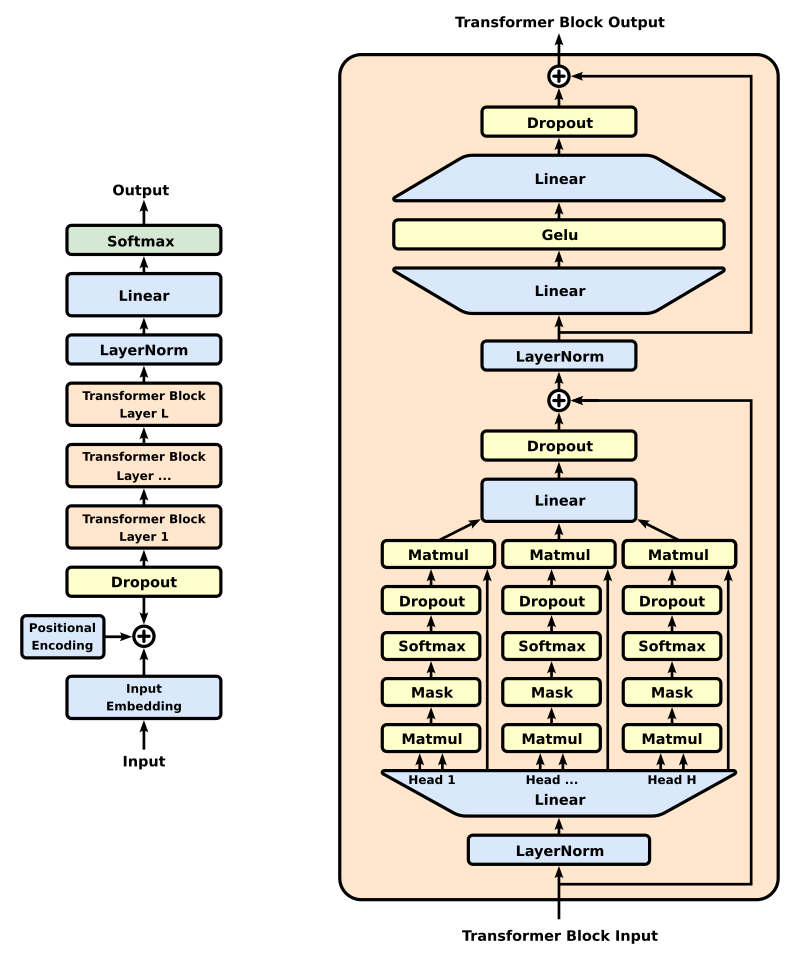
\includegraphics[width=0.8\columnwidth]{images/Full_GPT_architecture.png}
      \end{figure}
    \end{column}
  \end{columns}
\end{frame}

% Folie 3: Self-Attention Mechanismus
\begin{frame}{Self-Attention Mechanismus}
  \begin{columns}
    \begin{column}{0.5\textwidth}
      \begin{itemize}
        \item Jeder Token schaut auf andere Tokens in seinem Kontext (bisherige Tokens).
        \item GPT nutzt \textbf{Masked Multi-Head Self-Attention}, um die Vorhersage zukünftiger Tokens zu verhindern.
        \item Besteht aus:
          \begin{itemize}
            \item Lineare Transformationen zu Query, Key, Value
            \item Maskierung der Zukunft
            \item Softmax über Attention Scores
            \item Gewichtete Summation der Werte
          \end{itemize}
      \end{itemize}
    \end{column}
    \begin{column}{0.5\textwidth}
      \begin{figure}
        \centering
        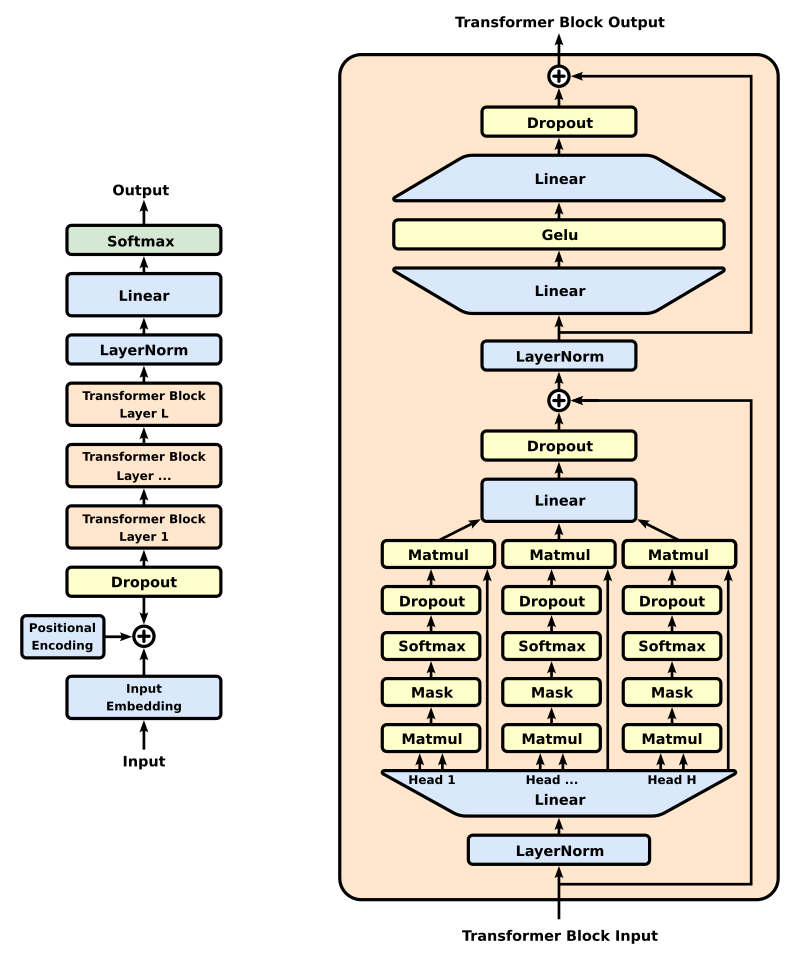
\includegraphics[width=0.8\columnwidth]{images/Full_GPT_architecture.png}
      \end{figure}
    \end{column}
  \end{columns}
\end{frame}

% Folie 4: Feedforward-Netz & Residual-Verbindungen
\begin{frame}{Feedforward-Netzwerk und Residual-Verbindungen}
  \begin{columns}
    \begin{column}{0.5\textwidth}
      \begin{itemize}
        \item Nach der Attention folgt ein Feedforward-Netz mit zwei linearen Schichten und einer Aktivierungsfunktion (GELU).
        
        \item GELU (Gaussian Error Linear Unit): Aktivierungsfunktion, definiert als:
          \[
          \text{GELU}(x) = x \cdot \Phi(x)
          \]
          wobei \(\Phi(x)\) die kumulative Verteilungsfunktion der Standardnormalverteilung ist:
          \[
          \Phi(x) = \frac{1}{2} \left( 1 + \text{erf}\left(\frac{x}{\sqrt{2}}\right) \right)
          \]
        \item Vorteil: Glattere Approximation im Vergleich zu ReLU, wodurch das Training stabiler wird.
        \item Residual-Verbindungen sorgen für stabileres Training.
        \item \textbf{LayerNorm} wird nach jeder Addition durchgeführt.
        \item \textbf{Dropout} wird zur Regularisierung verwendet.
      \end{itemize}
    \end{column}
    \begin{column}{0.5\textwidth}
      \begin{figure}
        \centering
        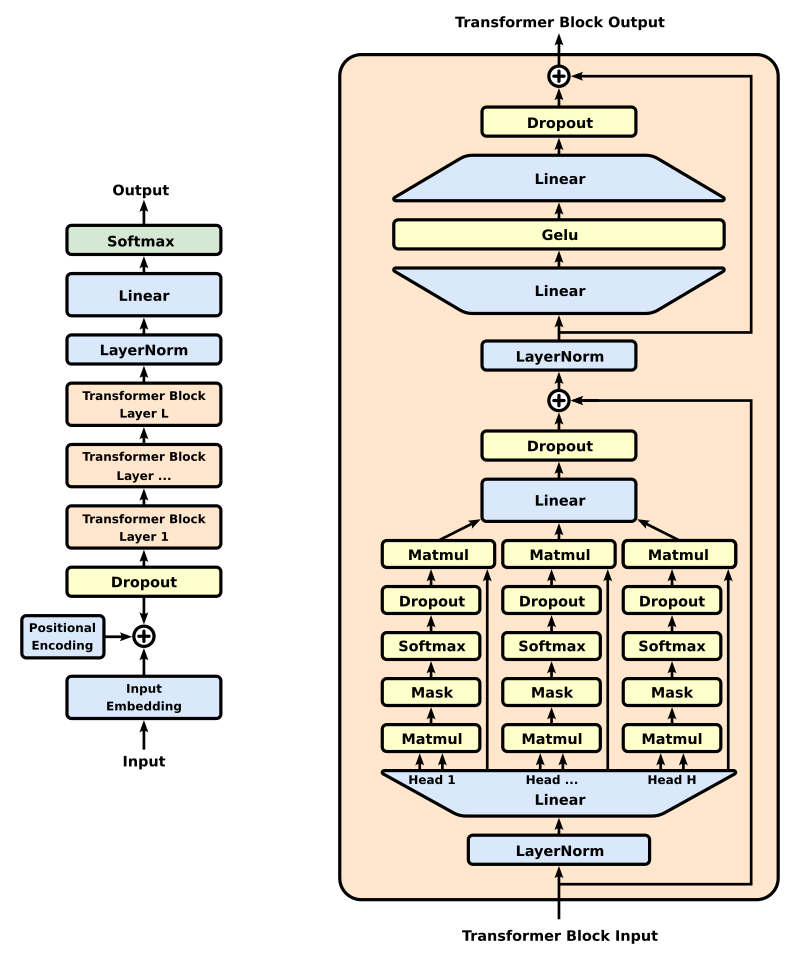
\includegraphics[width=0.8\columnwidth]{images/Full_GPT_architecture.png}
      \end{figure}
    \end{column}
  \end{columns}
\end{frame}

% Folie 5: Mehrere Transformer-Layer
\begin{frame}{Mehrere Transformer-Layer}
  \begin{columns}
    \begin{column}{0.5\textwidth}
      \begin{itemize}
        \item Die Blöcke werden L-mal gestapelt (z. B. 12 für GPT-2 small, 96 für GPT-3).
        \item Jeder Layer hat dieselbe Architektur.
        \item Die Ausgabe des letzten Blocks wird verwendet, um Token-Vorhersagen durch ein lineares Projektionslayer + Softmax zu erzeugen.
      \end{itemize}
    \end{column}
    \begin{column}{0.5\textwidth}
      \begin{figure}
        \centering
        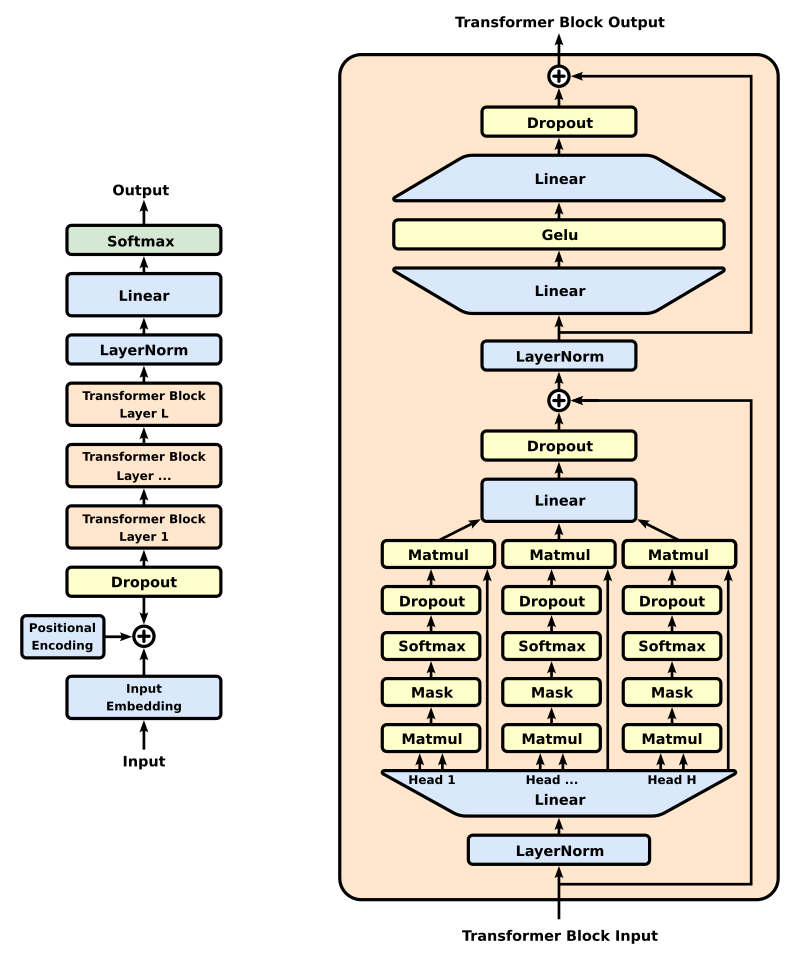
\includegraphics[width=0.8\columnwidth]{images/Full_GPT_architecture.png}
      \end{figure}
    \end{column}
  \end{columns}
\end{frame}

% Folie 6: Zusammenfassung
\begin{frame}{Zusammenfassung}
  \begin{columns}
    \begin{column}{0.5\textwidth}
      \begin{itemize}
        \item GPT besteht aus reinen Decoder-Blöcken des Transformers.
        \item Nutzt Masked Self-Attention zur autoregressiven Textgenerierung.
        \item Durch Pretraining auf sehr großen Textmengen kann GPT Sprachverständnis und -generierung erlernen.
      \end{itemize}
    \end{column}
    \begin{column}{0.5\textwidth}
      \begin{figure}
        \centering
        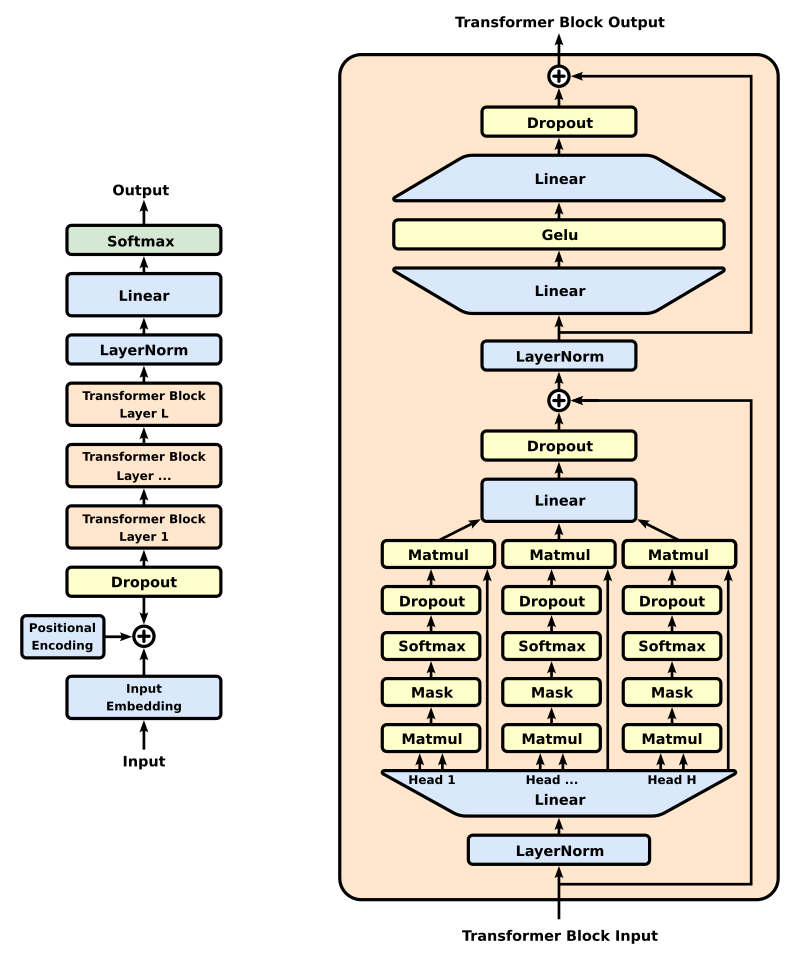
\includegraphics[width=0.8\columnwidth]{images/Full_GPT_architecture.png}
      \end{figure}
    \end{column}
  \end{columns}
\end{frame}

% Folie 7: Pretraining – Autoregressives Training
\begin{frame}{Pretraining: Autoregressives Training}
  \begin{itemize}
      \item GPT wird durch \textbf{Autoregressive Language Modeling} trainiert:
      \[
      P(x_1, x_2, ..., x_n) = \prod_{t=1}^{n} P(x_t \mid x_{<t})
      \]
      \item Ziel: Nächstes Token vorhersagen basierend auf bisherigen Tokens.
      \item Loss-Funktion: Kreuzentropie-Loss zwischen vorhergesagtem und wahrem nächsten Token.
      \item Kontext wird vollständig nach links maskiert.
  \end{itemize}
\end{frame}

% Folie 8: Trainingsdaten und Vorgehen
\begin{frame}{Trainingsdaten und Vorgehen}
  \begin{itemize}
      \item GPT wird auf großen Korpora wie Common Crawl, Wikipedia, Bücher, Webseiten etc. trainiert.
      \item Tokenisierung erfolgt meist mit Byte-Pair Encoding (BPE).
      \item Typische Trainingsparameter (für GPT-2):
      \begin{itemize}
          \item Kontextlänge: 1024 Tokens
          \item Batchgröße: mehrere Millionen Tokens
          \item Optimierung mit AdamW + Learning Rate Schedules
      \end{itemize}
      \item Kein spezieller Pretraining-Task wie bei BERT (z. B. Masked LM oder NSP).
  \end{itemize}
\end{frame}

% Folie 9: Fine-Tuning von GPT
\begin{frame}{Fine-Tuning von GPT}
  \begin{itemize}
      \item Nach dem Pretraining kann GPT für spezifische Aufgaben feinjustiert werden:
      \begin{itemize}
          \item Textklassifikation
          \item Fragebeantwortung
          \item Dialogsysteme
          \item Textgenerierung (z. B. ChatGPT)
      \end{itemize}
      \item Fine-Tuning erfolgt meist mit task-spezifischen Daten.
      \item Architektur bleibt gleich – es werden oft nur letzte Layer angepasst.
  \end{itemize}
\end{frame}


% Folie 10: GPT vs. BERT – Architektur und Trainingsziel
\begin{frame}{GPT vs. BERT – Fundamentale Unterschiede}
  \begin{columns}
      \column{0.48\textwidth}
      \textbf{GPT (Decoder-basiert)}
      \begin{itemize}
          \item Autoregressives Training (Zukunft maskiert)
          \item Nur Self-Attention nach links
          \item Einsatz: Textgenerierung, Dialogsysteme
          \item Output wird schrittweise erzeugt
      \end{itemize}
      
      \column{0.48\textwidth}
      \textbf{BERT (Encoder-basiert)}
      \begin{itemize}
          \item Masked Language Modeling (MLM)
          \item Bidirektionale Attention
          \item Einsatz: Klassifikation, Entitätenerkennung
          \item Kein autoregressiver Output
      \end{itemize}
  \end{columns}
  \vspace{0.4cm}
  \begin{center}
      \textit{GPT erzeugt Sprache -- BERT versteht sie.}
  \end{center}
\end{frame}

% Abschnitt: Fine-Tuning von LLMs
\section{Fine-Tuning von LLMs}

\begin{frame}{Was ist Fine-Tuning?}
  \begin{itemize}
    \item \textbf{Definition:} Anpassung eines vortrainierten Modells an eine spezifische Aufgabe oder Domäne.
    \item \textbf{Ziel:} Verbesserung der Leistung auf spezifischen Aufgaben durch zusätzliche Trainingsdaten.
    \item \textbf{Vorgehen:}
      \begin{itemize}
        \item Start mit einem vortrainierten Modell (z. B. BERT, GPT).
        \item Hinzufügen einer spezifischen Schicht (z. B. Klassifikationslayer).
        \item Training auf einem domänenspezifischen Datensatz.
      \end{itemize}
  \end{itemize}
\end{frame}

\begin{frame}{Vorteile des Fine-Tunings}
  \begin{itemize}
    \item \textbf{Effizienz:} Reduziert den Bedarf an großen Trainingsressourcen, da das Modell bereits vortrainiert ist.
    \item \textbf{Anpassungsfähigkeit:} Ermöglicht die Anpassung an spezifische Aufgaben oder Domänen.
    \item \textbf{Verbesserte Leistung:} Höhere Genauigkeit und Relevanz für spezifische Anwendungen.
    \item \textbf{Wiederverwendbarkeit:} Vortrainierte Modelle können für verschiedene Aufgaben wiederverwendet werden.
  \end{itemize}
\end{frame}

\begin{frame}{Nachteile des Fine-Tunings}
  \begin{itemize}
    \item \textbf{Overfitting:} Risiko, dass das Modell zu stark an den spezifischen Datensatz angepasst wird.
    \item \textbf{Datenbedarf:} Erfordert qualitativ hochwertige und ausreichend große Datensätze.
    \item \textbf{Rechenaufwand:} Kann trotz Vortraining immer noch ressourcenintensiv sein.
    \item \textbf{Komplexität:} Erfordert Fachwissen für die richtige Konfiguration und Optimierung.
  \end{itemize}
\end{frame}

% Abschnitt: Fine-Tuning-Techniken für LLMs
\section{Fine-Tuning-Techniken für LLMs}

\begin{frame}{Fine-Tuning-Techniken für LLMs}
  \begin{itemize}
    \item \textbf{Parameter-Efficient Fine-Tuning (PEFT):}
      \begin{itemize}
        \item Ziel: Reduktion der Anzahl der zu trainierenden Parameter.
        \item Vorteile: Geringerer Speicherbedarf und schnellere Trainingszeiten.
      \end{itemize}
    \item \textbf{Low-Rank Adaptation (LoRA):}
      \begin{itemize}
        \item Ziel: Effiziente Anpassung vortrainierter Modelle durch Low-Rank-Matrizen.
        \item Vorteile: Speicher- und Rechenaufwand werden drastisch reduziert.
      \end{itemize}
  \end{itemize}
\end{frame}

\begin{frame}{Parameter-Efficient Fine-Tuning (PEFT)}
  \begin{itemize}
    \item \textbf{Grundidee:}
      \begin{itemize}
        \item Statt das gesamte Modell zu aktualisieren, werden nur wenige Parameter angepasst.
        \item Nutzung von Adapter-Schichten, Prompt-Tuning oder LoRA.
      \end{itemize}
    \item \textbf{Mathematische Grundlage:}
      \begin{itemize}
        \item Gegeben ein vortrainiertes Modell mit Parametern \( \theta \).
        \item PEFT optimiert nur einen kleinen Teil \( \Delta \theta \), sodass:
          \[
          \theta' = \theta + \Delta \theta
          \]
        \item Ziel: Minimierung des Verlusts \( \mathcal{L} \) über \( \Delta \theta \):
          \[
          \min_{\Delta \theta} \mathcal{L}(f(x; \theta + \Delta \theta), y)
          \]
      \end{itemize}
    \item \textbf{Vorteile:}
      \begin{itemize}
        \item Reduktion des Speicherbedarfs.
        \item Wiederverwendbarkeit des vortrainierten Modells.
      \end{itemize}
  \end{itemize}
\end{frame}

\begin{frame}{Low-Rank Adaptation (LoRA): Grundidee}
  \begin{itemize}
    \item \textbf{Motivation:}
      \begin{itemize}
        \item Große Sprachmodelle haben Milliarden von Parametern.
        \item LoRA reduziert die Anzahl der zu trainierenden Parameter durch Low-Rank-Matrizen.
      \end{itemize}
    \item \textbf{Ansatz:}
      \begin{itemize}
        \item Zerlegung der Gewichtsmatrix \( W \) in zwei Low-Rank-Matrizen \( A \) und \( B \):
          \[
          W' = W + \Delta W, \quad \Delta W = A B^\top
          \]
        \item \( A \in \mathbb{R}^{d \times r} \), \( B \in \mathbb{R}^{d \times r} \), wobei \( r \ll d \).
      \end{itemize}
    \item \textbf{Vorteile:}
      \begin{itemize}
        \item Reduktion der Speicher- und Rechenkosten.
        \item Effizientes Fine-Tuning ohne Änderung der Hauptgewichte \( W \).
      \end{itemize}
  \end{itemize}
\end{frame}

\begin{frame}{Low-Rank Adaptation (LoRA): Mathematische Details}
  \begin{itemize}
    \item \textbf{Modellanpassung:}
      \begin{itemize}
        \item Gegeben eine Gewichtsmatrix \( W \), wird die Anpassung \( \Delta W \) durch:
          \[
          \Delta W = A B^\top
          \]
          berechnet, wobei \( A \) und \( B \) trainierbar sind.
      \end{itemize}
    \item \textbf{Optimierung:}
      \begin{itemize}
        \item Ziel: Minimierung des Verlusts \( \mathcal{L} \) über \( A \) und \( B \):
          \[
          \min_{A, B} \mathcal{L}(f(x; W + A B^\top), y)
          \]
      \end{itemize}
    \item \textbf{Effizienz:}
      \begin{itemize}
        \item Speicherbedarf: \( O(r \cdot (d + d)) \), wobei \( r \ll d \).
        \item Rechenaufwand: Geringer als vollständiges Fine-Tuning.
      \end{itemize}
  \end{itemize}
\end{frame}

\begin{frame}{Vergleich: PEFT, LoRA und Full Fine-Tuning}
  \begin{table}[]
    \centering
    \begin{tabular}{|l|l|l|l|}
      \hline
      \textbf{Eigenschaft} & \textbf{PEFT} & \textbf{LoRA} & \textbf{Full Fine-Tuning} \\ \hline
      Speicherbedarf & Gering & Sehr gering & Hoch \\ \hline
      Rechenaufwand & Mittel & Niedrig & Sehr hoch \\ \hline
      Flexibilität & Hoch & Mittel & Sehr hoch \\ \hline
      Anwendungsfälle & Allgemein & Speziell für LLMs & Universell \\ \hline
    \end{tabular}
    \caption{Vergleich von PEFT, LoRA und Full Fine-Tuning.}
  \end{table}
\end{frame}

\begin{frame}{Fine-Tuning Frameworks}
  \begin{itemize}
    \item \textbf{Hugging Face Transformers:}
      \begin{itemize}
        \item Umfangreiche Bibliothek für vortrainierte Modelle.
        \item Unterstützt einfache Anpassung und Fine-Tuning.
        \item \url{https://github.com/huggingface/transformers}
      \end{itemize}
    \item \textbf{OpenAI Fine-Tuning API:}
      \begin{itemize}
        \item Ermöglicht das Fine-Tuning von GPT-Modellen.
        \item Einfache Integration in bestehende Anwendungen.
        \item \url{https://platform.openai.com/docs/guides/fine-tuning}
      \end{itemize}
    \item \textbf{PyTorch Lightning:}
      \begin{itemize}
        \item Framework für vereinfachtes Training und Fine-Tuning.
        \item Unterstützt verteiltes Training und Mixed Precision.
        \item \url{https://www.pytorchlightning.ai/}
      \end{itemize}
    \item \textbf{LoRA (Low-Rank Adaptation):}
      \begin{itemize}
        \item Effizientes Fine-Tuning durch Reduktion der Parameteranzahl.
        \item Besonders geeignet für ressourcenbeschränkte Umgebungen.
        \item \url{https://github.com/microsoft/LoRA}
      \end{itemize}
  \end{itemize}
\end{frame}


% Abschnitt: Weitere LLM-Architekturen
\section{Weitere LLM-Architekturen}

\begin{frame}{GPT-2: Verbesserungen gegenüber GPT}
  \begin{itemize}
    \item \textbf{Größere Modelle:} GPT-2 wurde in verschiedenen Größen veröffentlicht (117M, 345M, 762M, 1.5B Parameter).
    \item \textbf{Training auf größeren Datenmengen:} GPT-2 wurde auf einem breiteren und vielfältigeren Korpus trainiert.
    \item \textbf{Verbesserte Textgenerierung:} GPT-2 erzeugt kohärentere und längere Texte.
    \item \textbf{Anwendungen:} Textzusammenfassung, Übersetzung, Dialogsysteme.
  \end{itemize}
\end{frame}

\begin{frame}{GPT-3: Skalierung und Few-Shot Learning}
  \begin{itemize}
    \item \textbf{Skalierung:} GPT-3 hat 175 Milliarden Parameter, was es zu einem der größten Modelle macht.
    \item \textbf{Few-Shot Learning:} Kann Aufgaben mit wenigen Beispielen im Prompt lösen.
    \item \textbf{Anwendungen:} Codegenerierung, kreative Textgenerierung, komplexe Dialoge.
    \item \textbf{Herausforderungen:} Hoher Rechenaufwand, Bias in den generierten Texten.
  \end{itemize}
\end{frame}

\begin{frame}{GPT-4: Multimodalität und Verbesserungen}
  \begin{itemize}
    \item \textbf{Multimodalität:} GPT-4 kann sowohl Text als auch Bilder als Eingabe verarbeiten.
    \item \textbf{Verbesserte Genauigkeit:} Bessere Leistung bei komplexen Aufgaben und längeren Kontexten.
    \item \textbf{Anwendungen:} Bildbeschreibung, multimodale Dialogsysteme.
    \item \textbf{Herausforderungen:} Noch höhere Anforderungen an Rechenressourcen.
  \end{itemize}
\end{frame}

\begin{frame}{GPT-4: Multimodale Verarbeitung}
  \begin{itemize}
    \item \textbf{Multimodalität:} GPT-4 kann sowohl Text als auch Bilder als Eingabe verarbeiten.
    \item \textbf{Architektur:}
      \begin{itemize}
        \item Erweiterung der Transformer-Architektur, um visuelle und textuelle Daten zu integrieren.
        \item Gemeinsamer latent space für Text- und Bildrepräsentationen.
      \end{itemize}
    \item \textbf{Anwendungen:}
      \begin{itemize}
        \item Bildbeschreibung: Generierung von Texten basierend auf Bildern.
        \item Visuelle Fragebeantwortung: Beantwortung von Fragen zu einem Bild.
        \item Multimodale Dialogsysteme: Kombination von Text- und Bildinformationen in Konversationen.
      \end{itemize}
  \end{itemize}
\end{frame}

\begin{frame}{GPT-4: Verarbeitung von Bildern und Text}
  \begin{itemize}
    \item \textbf{Bildverarbeitung:}
      \begin{itemize}
        \item Bilder werden durch ein visuelles Encoder-Modul (z. B. CNN oder Vision Transformer) in Features umgewandelt.
        \item Die Features werden in den Transformer integriert.
      \end{itemize}
    \item \textbf{Textverarbeitung:}
      \begin{itemize}
        \item Text wird wie in GPT-3 tokenisiert und in Embeddings umgewandelt.
        \item Gemeinsame Verarbeitung mit Bild-Features im Transformer.
      \end{itemize}
  \end{itemize}
  \begin{figure}
    \centering
      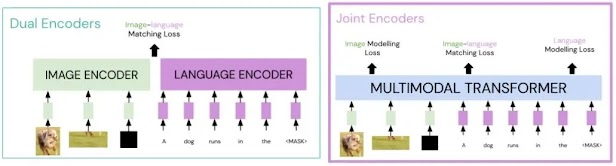
\includegraphics[width=0.8\textwidth]{images/multimodal.jpg}
      \caption{Multimodale Verarbeitung in Language models\footnote{\url{https://lh3.googleusercontent.com/UGw_gUAQ0ja_28B-s-o0othiI2rmsIO2WJ_48s0xapPIfYJwK-pof8TgOqwnQwI0h4t6-RUw6saGjjWUDpqC224WwIPnnpiBfqa5fLiKbsURczSwDGw=w616}}}
  \end{figure}
\end{frame}

\begin{frame}{GPT-4: Herausforderungen und Vorteile}
  \begin{itemize}
    \item \textbf{Herausforderungen:}
      \begin{itemize}
        \item Integration von Bild- und Textdaten in einem Modell.
        \item Hoher Rechenaufwand für Training und Inferenz.
        \item Bedarf an großen multimodalen Datensätzen.
      \end{itemize}
    \item \textbf{Vorteile:}
      \begin{itemize}
        \item Verbesserte Kontextverständnis durch Kombination von Text und Bild.
        \item Breitere Anwendungsbereiche, z. B. in der Medizin, Bildung und Unterhaltung.
        \item Fortschritt in multimodalen KI-Systemen.
      \end{itemize}
  \end{itemize}
\end{frame}

\begin{frame}{LLaMA: Open-Weight Modelle}
  \begin{itemize}
    \item \textbf{LLaMA (Large Language Model Meta AI):} Entwickelt von Meta AI, mit Fokus auf Effizienz und Zugänglichkeit.
    \item \textbf{Open-Weight Modelle:} Verfügbar für die Forschungsgemeinschaft.
    \item \textbf{Größen:} Modelle mit 7B, 13B, 30B und 70B Parametern.
    \item \textbf{Anwendungen:} Forschung, Entwicklung von spezialisierten LLMs.
  \end{itemize}
\end{frame}

% Abschnitt: Neuartige Reasoning-Modelle
\section{Neuartige Reasoning-Modelle}

\begin{frame}{Einführung in Reasoning-Modelle}
  \begin{itemize}
    \item Reasoning-Modelle zielen darauf ab, logisches Denken und Schlussfolgerungen zu ermöglichen.
    \item Fokus auf komplexe Aufgaben wie mathematische Beweise, logische Schlussfolgerungen und Multi-Hop-Fragen.
    \item Beispiele: DeepSeek-r1, GPT4o, DeepMind Gemini, Anthropic Claude.
  \end{itemize}
\end{frame}

\begin{frame}{DeepSeek-r1: Überblick}
  \begin{itemize}
    \item \textbf{DeepSeek-r1:} Ein neuartiges Reasoning-Modell, das auf Transformer-Architekturen basiert.
    \item \textbf{Ziele:}
      \begin{itemize}
        \item Integration von logischem Denken in Sprachmodelle.
        \item Dieses Reasoning imitiert menschliches Denken über Generierung von Tokens
        \item Verarbeitung von Multi-Hop-Reasoning-Aufgaben.
        \item Unterstützung von domänenspezifischen Schlussfolgerungen.
      \end{itemize}
    \item \textbf{Besonderheiten:}
      \begin{itemize}
        \item Hybrid-Architektur mit dedizierten Reasoning-Modulen.
        \item Nutzung von Memory-Augmented Mechanismen.
      \end{itemize}
  \end{itemize}
\end{frame}

\begin{frame}{DeepSeek-r1: Architektur}
  \begin{itemize}
    \item \textbf{Core-Komponenten:}
      \begin{itemize}
        \item \textbf{Reasoning-Module:} Spezialisierte Submodule für logische Schlussfolgerungen.
        \item \textbf{Memory-Augmented Attention:} Ermöglicht Zugriff auf externe Wissensquellen.
        \item \textbf{Multi-Hop-Mechanismus:} Iterative Verarbeitung von Informationen.
      \end{itemize}
    \item \textbf{Pipeline:}
      \begin{enumerate}
        \item Eingabe wird tokenisiert und in Embeddings umgewandelt.
        \item Reasoning-Module führen "logische" Operationen durch.
        \item Ergebnisse werden iterativ verfeinert.
        \item Ausgabe erfolgt als Schlussfolgerung oder Antwort.
      \end{enumerate}
  \end{itemize}
\end{frame}

\begin{frame}{Überblick DeepSeek-R1}
  \begin{itemize}
      \item \textbf{Ziel:} Maximale Ausnutzung von Test-Time Computation zur Förderung von Ketten- bzw. Chain-of-Thought (CoT) Reasoning.
      \item DeepSeek-R1 erreicht ähnliche Leistungen wie GPT-o1, jedoch mit deutlich geringeren Trainingskosten.
      \item Einsatz von Reinforcement Learning (RL) als dominanter Post-Training-Ansatz, um komplexe Reasoning-Aufgaben (Mathematik, Code, wissenschaftliches Denken) zu meistern.
  \end{itemize}
\end{frame}

% Folie 3: Architekturdetails
\begin{frame}{Architektur von DeepSeek-R1}
  \begin{itemize}
    \item Basierend auf einem DeepSeek-V3-Base Checkpoint.
    \item Nutzt \textbf{Mixture-of-Expert (MoE)}-Strukturen, Multi-Head Latent Attention (MLA) und Multi-Token Prediction (MTP).
    \item Zwei Varianten:
    \begin{itemize}
        \item \textbf{DeepSeek-R1-Zero:} Post-Training ausschließlich mit RL.
        \item \textbf{DeepSeek-R1:} Mehrstufiger Post-Training-Prozess, der zusätzlich Supervised Fine-Tuning (SFT) integriert.
    \end{itemize}
    \end{itemize}
    \begin{center}
      \begin{figure}
        \centering
        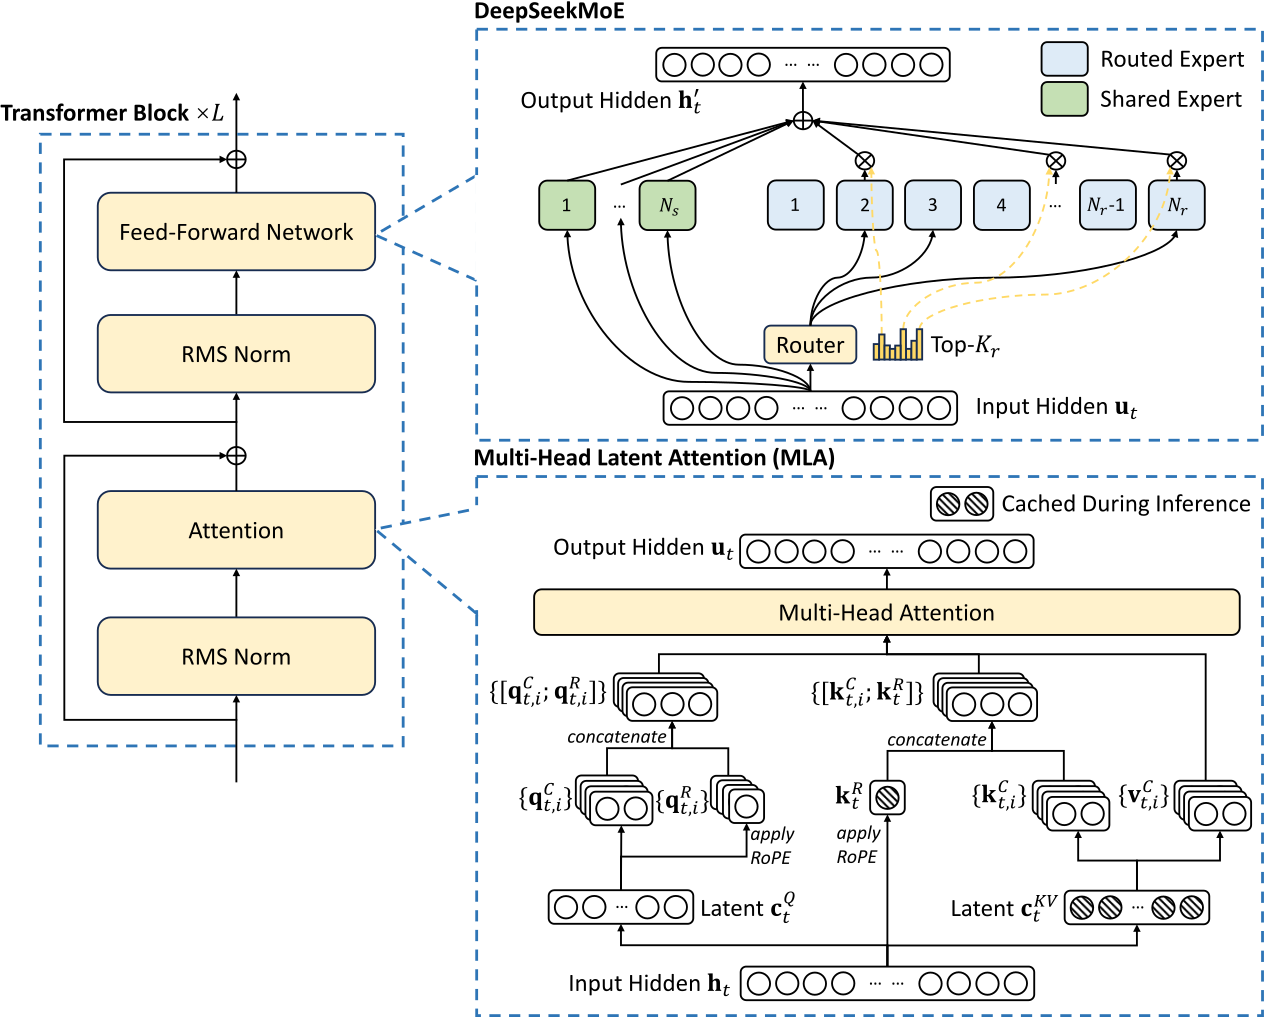
\includegraphics[width=0.6\textwidth]{images/DeepSeek_MoE_and_MLA_(DeepSeek-V2).png}
        \caption{DeepSeek MoE and MLA Architecture (DeepSeek-V2).}
      \end{figure}
    \end{center}
\end{frame}

% Abschnitt: Mathematische Grundlagen
\section{Mathematische Grundlagen}

\begin{frame}{Proximal Policy Optimization (PPO) - Teil 1}
  \begin{itemize}
    \item \textbf{Definition:} PPO ist ein Reinforcement-Learning-Algorithmus, der die Policy-Gradient-Methode verbessert.
    \item \textbf{Ziel:} Maximierung der kumulierten Belohnung durch Optimierung der Policy \( \pi_\theta \).
    \item \textbf{Kernidee:} Begrenzung der Policy-Änderungen, um Stabilität und Effizienz zu gewährleisten.
    \item \textbf{Details:} \url{https://arxiv.org/pdf/2402.03300}
  \end{itemize}
  \vspace{0.5cm}
  \textbf{PPO-Zielfunktion:}
  \[
  L^{\mathrm{CLIP}}(\theta) = \mathbb{E}_t \left[ \min \left( r_t(\theta) \hat{A}_t, \mathrm{clip}(r_t(\theta), 1-\epsilon, 1+\epsilon) \hat{A}_t \right) \right]
  \]
\end{frame}

\begin{frame}{Proximal Policy Optimization (PPO) - Teil 2}
  \begin{itemize}
    \item \( r_t(\theta) = \frac{\pi_\theta(a_t|s_t)}{\pi_{\theta_{\text{old}}}(a_t|s_t)} \): Verhältnis der neuen zur alten Policy.
    \item \( \hat{A}_t \): Vorteil (Advantage) zur Zeit \( t \).
    \item \( \epsilon \): Hyperparameter zur Begrenzung der Policy-Änderung.
  \end{itemize}
  \vspace{0.5cm}
  \textbf{Vorteile von PPO:}
  \begin{itemize}
    \item Stabilität durch Clipping der Policy-Änderungen.
    \item Einfache Implementierung und gute Leistung in verschiedenen RL-Aufgaben.
  \end{itemize}
\end{frame}

% Folie 4: GRPO – Der RL-Algorithmus
\begin{frame}{GRPO – Group Relative Policy Optimization (Teil 1)}
  \begin{itemize}
      \item DeepSeek-R1 setzt auf eine modifizierte Version von PPO namens \textbf{Group Relative Policy Optimization (GRPO)}.
      \item Ziel: Steigerung der mathematischen Reasoning-Fähigkeiten bei reduziertem Speicherverbrauch.
  \end{itemize}
  \vspace{0.3cm}
  \textbf{GRPO Objective:}\\[0.2cm]
  Die GRPO-Ziel-Funktion basiert auf der PPO-Formulierung:
  \[
  L^{\mathrm{CLIP}}(\theta) = \mathbb{E}_{t} \left[ \min \left( r_{t}(\theta) \,\hat{A}_{t},\, \mathrm{clip}\left(r_{t}(\theta), 1-\epsilon, 1+\epsilon \right) \,\hat{A}_{t} \right) \right]
  \]
  wobei:
  \begin{itemize}
      \item \( r_{t}(\theta) = \frac{\pi_{\theta}(a_t|s_t)}{\pi_{\theta_{\mathrm{old}}}(a_t|s_t)} \) ist der Wahrscheinlichkeitsquotient.
      \item \( \hat{A}_{t} \) bezeichnet den Vorteil (Advantage) zur Zeit \( t \).
      \item \( \epsilon \) ist ein Hyperparameter zur Begrenzung der Änderung.
  \end{itemize}
\end{frame}

\begin{frame}{GRPO – Group Relative Policy Optimization (Teil 2)}
  \textbf{Gruppenbezogene Anpassungen:}\\[0.2cm]
  GRPO erweitert die PPO-Zielfunktion, indem es gruppenspezifische Gewichtungen einführt:
  \[
  L^{\mathrm{GRPO}}(\theta) = \mathbb{E}_{t, g} \left[ \min \left( r_{t,g}(\theta) \,\hat{A}_{t,g},\, \mathrm{clip}\left(r_{t,g}(\theta), 1-\epsilon, 1+\epsilon \right) \,\hat{A}_{t,g} \right) \right]
  \]
  wobei:
  \begin{itemize}
      \item \( g \) die Gruppe repräsentiert, zu der die Aufgabe gehört.
      \item \( r_{t,g}(\theta) = \frac{\pi_{\theta}(a_t|s_t, g)}{\pi_{\theta_{\mathrm{old}}}(a_t|s_t, g)} \) ist der gruppenspezifische Wahrscheinlichkeitsquotient.
      \item \( \hat{A}_{t,g} \) ist der gruppenspezifische Vorteil (Advantage).
  \end{itemize}
  Diese Erweiterung ermöglicht es, die Policy-Optimierung an die spezifischen Anforderungen und Eigenschaften verschiedener Gruppen anzupassen, wodurch die Leistung in heterogenen Aufgabenbereichen verbessert wird.
\end{frame}

\begin{frame}{GRPO – Group Relative Policy Optimization (Teil 3)}
  \begin{columns}
    \begin{column}{0.5\textwidth}
      \begin{itemize}
        \item \textbf{Visualisierung:} Die folgende Abbildung illustriert die Funktionsweise von GRPO.
        \item \textbf{Schlüsselkonzepte:}
          \begin{itemize}
            \item Gruppenspezifische Gewichtungen.
            \item Begrenzung der Policy-Änderungen.
            \item Iterative Optimierung für verschiedene Gruppen.
          \end{itemize}
      \end{itemize}
    \end{column}
    \begin{column}{0.5\textwidth}
      \begin{figure}
        \centering
        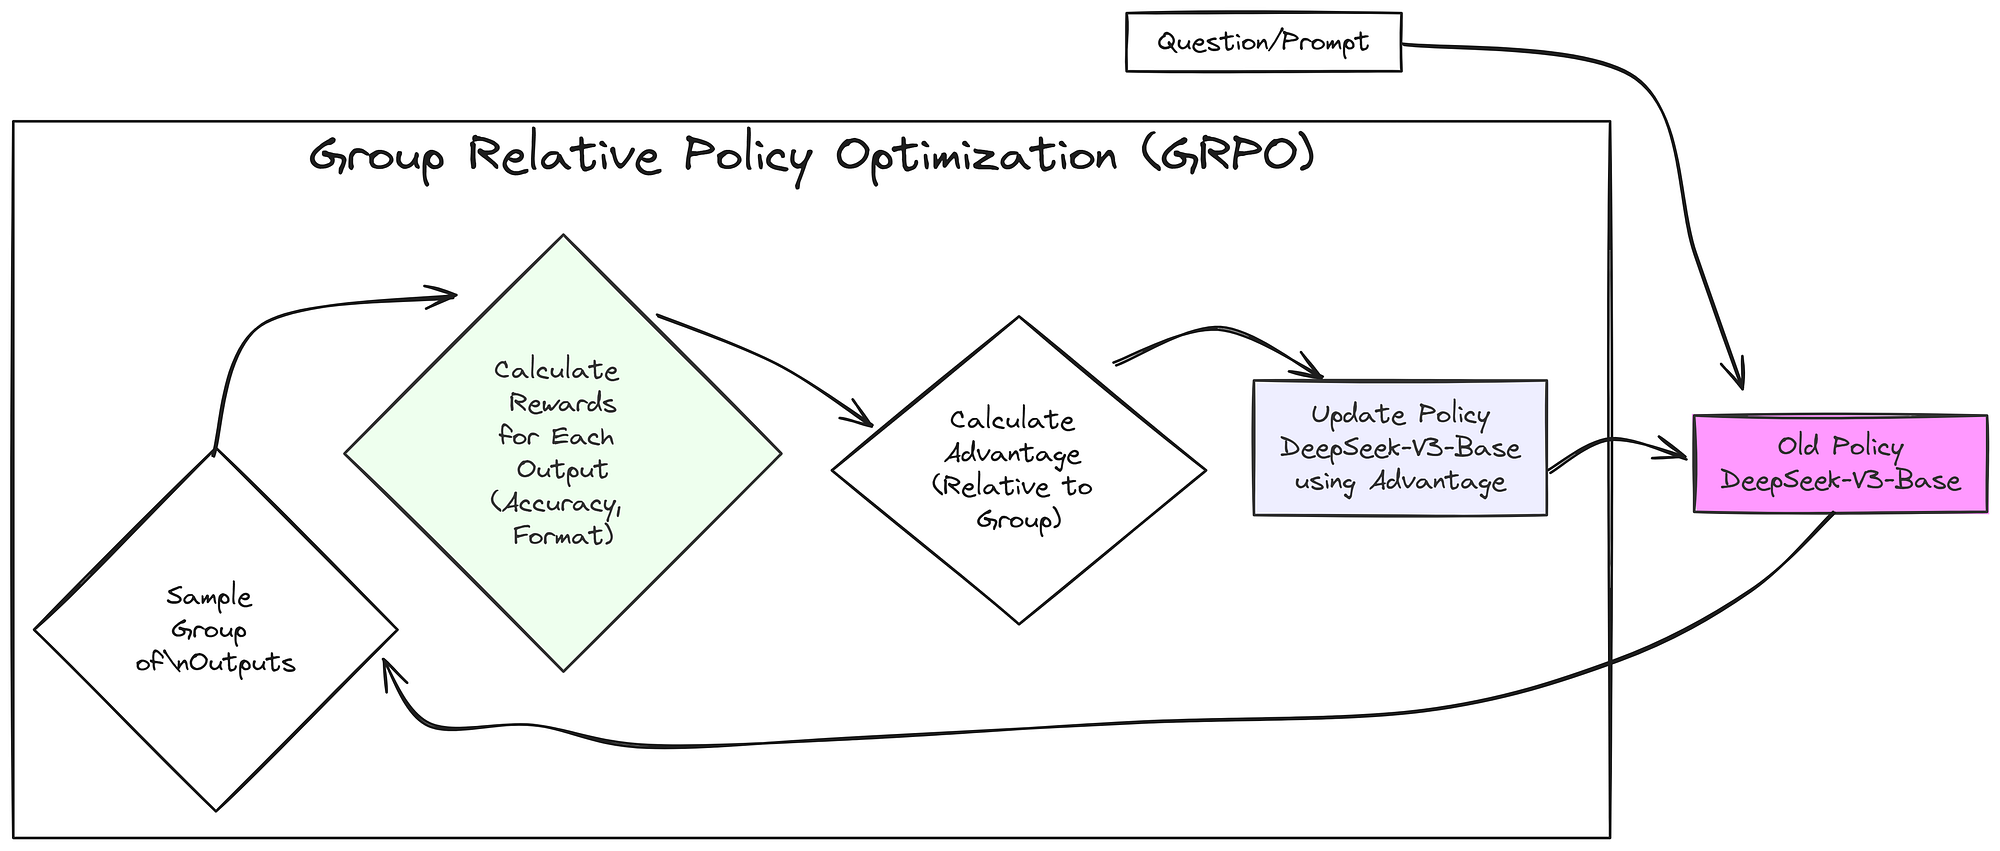
\includegraphics[width=\textwidth]{images/GRPO.png}
        \caption{Illustration der GRPO-Mechanik.}
      \end{figure}
    \end{column}
  \end{columns}
\end{frame}

% Folie 5: Reward-Modellierung
\begin{frame}{Reward-Modellierung}
  \begin{itemize}
      \item \textbf{Regelbasierte Rewards:}
      \begin{itemize}
          \item \textbf{Accuracy Reward:} Bewertet, ob die Antwort korrekt ist.
          \item \textbf{Format Reward:} Erzwingt, dass der Denkprozess in \texttt{<think>} und \texttt{</think>} Tags eingeschlossen wird.
      \end{itemize}
      \item Kein neutral trainierter Reward Model, da solche Modelle anfällig für \emph{Reward Hacking} sind.
  \end{itemize}
  \vspace{0.3cm}
  \textbf{Kombinierter Reward:}\\[0.2cm]
  \[
  R_{\mathrm{total}} = \alpha\, R_{\mathrm{accuracy}} + \beta\, R_{\mathrm{format}}
  \]
  \begin{itemize}
      \item \(\alpha\) und \(\beta\) sind Gewichtungsfaktoren, die den Einfluss der jeweiligen Komponenten steuern.
  \end{itemize}
\end{frame}

% Folie 6: Mehrstufiger Trainingsprozess
\begin{frame}{Mehrstufiger Trainingsprozess von DeepSeek-R1}
  \begin{enumerate}
      \item \textbf{Phase 1: Cold-Start SFT}
          \begin{itemize}
              \item Erste Supervised Fine-Tuning (SFT) Phase, bei der Labels durch wenige Beispiele von R1-Zero generiert und von Menschen verfeinert werden.
          \end{itemize}
      \item \textbf{Phase 2: Reinforcement Learning}
          \begin{itemize}
              \item Anwendung von GRPO zur Optimierung der Reasoning-Fähigkeiten.
              \item Mathematische Zielsetzung zur Maximierung der Test-Time Computation: Der durchschnittliche Antwortlänge-Wert steigt, was eine tiefergehende Ketten-Denke (Chain-of-Thought) anzeigt.
          \end{itemize}
      \item \textbf{Phase 3: Weitere SFT}
          \begin{itemize}
              \item Integration von Daten aus weiteren Domänen zur Verbesserung von Schreibstil, Rollenspiel und allgemeinen Aufgaben.
          \end{itemize}
      \item \textbf{Phase 4: Sekundäres RL}
          \begin{itemize}
              \item RL für alle Szenarien zur Steigerung der Hilfsbereitschaft und Harmlosigkeit.
          \end{itemize}
  \end{enumerate}
\end{frame}

% Folie 7: Chain-of-Thought und Test-Time Computation
\begin{frame}{Chain-of-Thought und Test-Time Computation}
  \begin{itemize}
      \item DeepSeek-R1 nutzt \textbf{Chain-of-Thought (CoT)}-Reasoning:
          \begin{itemize}
              \item Zuerst wird ein ausführlicher Denkprozess (innerhalb von \texttt{<think>} … \texttt{</think>} Tags) generiert.
              \item Anschließend wird die finale Antwort produziert.
          \end{itemize}
      \item Mathematische Modellierung dieser Phase kann als iterative Optimierung über Teilschritte betrachtet werden, z.B.:
          \[
          \mathbf{c}_{t+1} = f(\mathbf{c}_t, \Delta_t(\mathbf{x}))
          \]
          wobei \(\mathbf{c}_t\) den aktuellen CoT-Zustand und \(\Delta_t(\mathbf{x})\) den Beitrag des nächsten Tokens bzw. der nächsten Denkschritt repräsentiert.
      \item Durch längeres Denken bei steigender Testzeit skaliert die Modellleistung im Sinne der "Test-time Scaling Law".
  \end{itemize}
\end{frame}

% Folie 8: Zusammenfassung und Ausblick
\begin{frame}{Zusammenfassung}
  \begin{itemize}
      \item DeepSeek-R1 demonstriert, wie Reinforcement Learning (GRPO) und regelbasierte Reward-Strategien genutzt werden können, um komplexe reasoning-Aufgaben zu bewältigen.
      \item Der mehrstufige Trainingsprozess (SFT $\rightarrow$ RL $\rightarrow$ SFT $\rightarrow$ RL) verbessert sowohl die Genauigkeit als auch die Sprachkohärenz.
      \item Die mathematische Grundlage der GRPO-Ziel-Funktion und der Reward-Modellierung zeigen, wie Optimierungsziele systematisch in den Trainingsprozess integriert werden.
  \end{itemize}
  \vspace{0.3cm}
  \begin{center}
      \textit{DeepSeek-R1 zeigt: Mit reduzierten Trainingskosten und innovativen Trainingsansätzen sind moderne Reasoning-Modelle möglich.}
  \end{center}
\end{frame}

\begin{frame}{Zusammenfassung: DeepSeek-r1 und LLM-Architekturen}
  \begin{itemize}
    \item \textbf{DeepSeek-r1:}
      \begin{itemize}
        \item Hervorragende Reasoning-Fähigkeiten und Multi-Hop-Reasoning.
        \item Zugriff auf externen Speicher für komplexe Schlussfolgerungen.
        \item Anwendungen: Logik, Beweise, domänenspezifische Aufgaben.
      \end{itemize}
    \item \textbf{Vergleich von LLMs:}
      \begin{itemize}
        \item GPT-2: Verbesserte Textgenerierung, Anwendungen wie Textzusammenfassung.
        \item GPT-3: 175B Parameter, Few-Shot Learning, z. B. Codegenerierung.
        \item GPT-4: Multimodalität (Text und Bild), Anwendungen wie Bildbeschreibung.
        \item LLaMA: Open-Weight Modelle (7B-70B Parameter), Fokus auf Forschung.
        \item DeepSeek-v3: Fortschrittliche Reasoning- und Domänenanpassungsfähigkeiten, Anwendungen in Wissenschaft und Technik.
      \end{itemize}
  \end{itemize}
\end{frame}


% Abschnitt 6: Zukunftsperspektiven
\section{Und was machen wir jetzt mit diesen Systemen?}

\begin{frame}{Und was machen wir jetzt mit diesen Systemen?}
  \begin{itemize}
    \item Praktische Anwendungen und Integration in bestehende Systeme \\
    \item Herausforderungen bei der Implementierung und Skalierung \\
    \item Gesellschaftliche und ethische Implikationen
  \end{itemize}
\end{frame}

% Abschnitt 7: Nutzungsmöglichkeiten: RAG, Agentensysteme
\section{Nutzungsmöglichkeiten: RAG, Agentensysteme}

\begin{frame}{Nutzungsmöglichkeiten: RAG, Agentensysteme}
  \begin{itemize}
    \item Retrieval-Augmented Generation (RAG) und seine Anwendungen \\
    \item Entwicklung und Einsatz von Agentensystemen im NLP \\
    \item Kombination von LLMs mit externem Wissen
  \end{itemize}
\end{frame}

\section{Retrieval-Augmented Generation (RAG)}

\begin{frame}{Was ist Retrieval-Augmented Generation (RAG)?}
  \begin{itemize}
    \item \textbf{Definition:} Kombination von Retrieval-Systemen und generativen Modellen.
    \item \textbf{Ziel:} Verbesserung der Antwortqualität durch Zugriff auf externe Wissensquellen.
    \item \textbf{Funktionsweise:}
      \begin{itemize}
        \item Abruf relevanter Dokumente aus einer Wissensdatenbank.
        \item Nutzung der abgerufenen Informationen zur Generierung von Antworten.
      \end{itemize}
    \item \textbf{Anwendungen:} Fragebeantwortung, Chatbots, Dokumentensuche.
  \end{itemize}
\end{frame}

\begin{frame}{RAG: Architektur}
  \begin{itemize}
    \item \textbf{Retriever:}
      \begin{itemize}
        \item Abruf relevanter Dokumente aus einer Wissensdatenbank. \\
        \item Nutzung von Suchalgorithmen und Vektorraumsmodellen.
      \end{itemize}

  \end{itemize}
  \begin{figure}
    \centering
    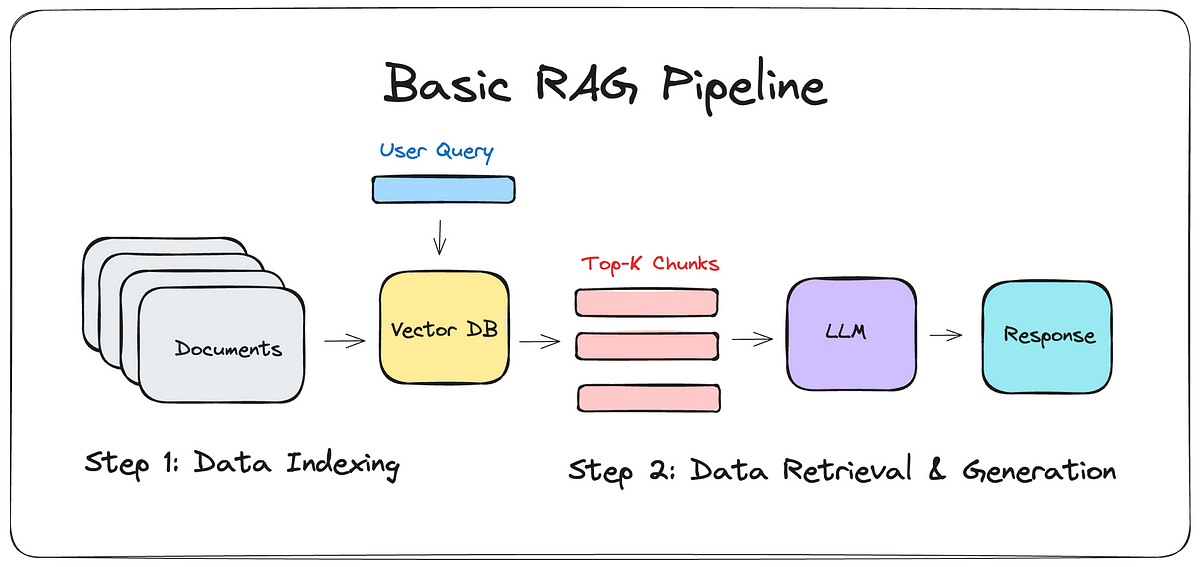
\includegraphics[width=0.8\textwidth]{images/basicrag.png}
    \caption{RAG-Architektur\footnote{https://medium.com/@drjulija/what-is-retrieval-augmented-generation-rag-938e4f6e03d1}}
  \end{figure}
\end{frame}

\begin{frame}{RAG: Vorteile}
  \begin{itemize}
    \item \textbf{Verbesserte Genauigkeit:} Zugriff auf externe Wissensquellen reduziert Halluzinationen. \\
    \item \textbf{Flexibilität:} Kann mit verschiedenen Retrieval- und Generationsmodellen kombiniert werden. \\
    \item \textbf{Aktualität:} Ermöglicht die Nutzung aktueller Informationen aus einer Wissensdatenbank. \\
    \item \textbf{Erweiterbarkeit:} Einfaches Hinzufügen neuer Wissensquellen.
  \end{itemize}
\end{frame}

\begin{frame}{RAG: Herausforderungen}
  \begin{itemize}
    \item \textbf{Effizienz:} Abruf und Generierung können rechenintensiv sein. \\
    \item \textbf{Schnittstellen:} Legacy-Systeme und APIs müssen integriert werden. \\
    \item \textbf{Access Rights Management:} Sicherstellen, dass nur autorisierte Informationen abgerufen werden. \\
    \item \textbf{Qualität der Dokumente:} Die Genauigkeit hängt von der Qualität der abgerufenen Dokumente ab. \\
    \item \textbf{Konsistenz:} Inkonsistenzen zwischen abgerufenen Informationen und generierten Antworten. \\
    \item \textbf{Bias:} Bias in der Wissensdatenbank können die Antworten beeinflussen.
  \end{itemize}
\end{frame}

\begin{frame}{RAG: Anwendungen}
  \begin{itemize}
    \item \textbf{Fragebeantwortung:} Beantwortung komplexer Fragen durch Abruf relevanter Informationen. \\
    \item \textbf{Chatbots:} Verbesserung der Konversationsqualität durch Zugriff auf externe Daten. \\
    \item \textbf{Dokumentensuche:} Generierung von Zusammenfassungen basierend auf abgerufenen Dokumenten. \\
    \item \textbf{Wissenschaftliche Recherche:} Unterstützung bei der Suche nach relevanter Literatur.
  \end{itemize}
\end{frame}

% Abschnitt: Document Embedding
\section{Document Embedding in RAG Pipelines}

\begin{frame}{Was ist Document Embedding in RAG Pipelines?}
  \begin{itemize}
    \item \textbf{Definition:} Repräsentation eines gesamten Dokuments/Chunks als Vektor in einem kontinuierlichen Vektorraum, speziell für Retrieval-Augmented Generation (RAG).
    \item \textbf{Ziel:} Ermöglichen eines effizienten Abrufs relevanter Dokumente/Chunks aus einer Vektordatenbank.
    \item \textbf{Anwendungen in RAG:}
      \begin{itemize}
        \item Verbesserung der Antwortqualität durch Zugriff auf relevante Dokumente.
        \item Unterstützung von Fragebeantwortung und Dokumentensuche.
        \item Integration von externem Wissen in generative Modelle.
      \end{itemize}
  \end{itemize}
\end{frame}

\begin{frame}{Strategien für Document Embedding in RAG Pipelines}
  \begin{itemize}
    \item \textbf{Transformer-basierte Modelle:}
      \begin{itemize}
        \item Nutzung von Modellen wie Sentence-BERT, OpenAI Embeddings oder ähnliche.
        \item CLS-Token oder Mittelung der Token-Embeddings für die Dokumentrepräsentation.
        \item Vorteile: Kontextabhängige und semantisch reichhaltige Repräsentationen.
      \end{itemize}
    \item \textbf{Vektordatenbanken:}
      \begin{itemize}
        \item Speicherung der Dokumentvektoren in spezialisierten Datenbanken wie Pinecone, Weaviate oder Milvus.
        \item Ermöglichen schnellen Abruf durch Ähnlichkeitssuche (z. B. k-NN, cosine similarity).
      \end{itemize}
    \item \textbf{Hybrid-Ansätze:}
      \begin{itemize}
        \item Kombination von klassischen Retrieval-Methoden (z. B. BM25) mit Vektorbasierter Suche.
        \item Verbesserung der Präzision durch Kombination von Semantik und Schlüsselwortsuche.
      \end{itemize}
  \end{itemize}
\end{frame}

\begin{frame}{Einbettung in Vektordatenbanken für RAG Pipelines}
  \begin{itemize}
    \item \textbf{Pipeline:}
      \begin{enumerate}
        \item Dokumente werden vorverarbeitet und in Vektoren eingebettet. \\
        \item Die Vektoren werden in einer Vektordatenbank gespeichert.\\
        \item Bei einer Anfrage wird der Eingabetext ebenfalls eingebettet. \\
        \item Ähnlichkeitssuche in der Vektordatenbank liefert relevante Dokumente. \\
        \item Die abgerufenen Dokumente werden als Kontext für die Generierung verwendet. 
      \end{enumerate}
    \item \textbf{Vorteile:}
      \begin{itemize}
        \item Effiziente Suche in großen Wissensbasen.
        \item Kontextualisierte Antworten durch semantische Relevanz.
        \item Skalierbarkeit für umfangreiche Datenmengen.
      \end{itemize}
  \end{itemize}
\end{frame}


\begin{frame}{Hybride Suche: BM25 und Vektorähnlichkeiten (Teil 1)}
  \begin{itemize}
    \item \textbf{Definition:} Kombination von klassischen Suchmethoden (BM25) und vektorbasierter Ähnlichkeitssuche.
    \item \textbf{BM25:}
      \begin{itemize}
        \item Klassischer Algorithmus für die Schlüsselwortsuche.
        \item Bewertet die Relevanz eines Dokuments basierend auf Termfrequenz (TF) und inverser Dokumentfrequenz (IDF).
        \item Formel:
          \[
          \text{BM25}(q, d) = \sum_{t \in q} \text{IDF}(t) \cdot \frac{f(t, d) \cdot (k_1 + 1)}{f(t, d) + k_1 \cdot (1 - b + b \cdot \frac{|d|}{\text{avgdl}})}
          \]
          wobei \( f(t, d) \) die Häufigkeit des Terms \( t \) im Dokument \( d \) ist.
      \end{itemize}
    \item \textbf{Vektorähnlichkeiten:}
      \begin{itemize}
        \item Repräsentiert Dokumente und Anfragen als Vektoren in einem kontinuierlichen Raum.
        \item Nutzt Metriken wie Kosinus-Ähnlichkeit oder euklidische Distanz zur Bewertung der Relevanz.
      \end{itemize}
  \end{itemize}
\end{frame}

\begin{frame}{Hybride Suche: BM25 und Vektorähnlichkeiten (Teil 2)}
  \begin{itemize}
    \item \textbf{Kombination:}
      \begin{itemize}
        \item BM25 liefert eine gewichtete Bewertung basierend auf Schlüsselwörtern.
        \item Vektorähnlichkeiten ergänzen die Suche durch semantische Relevanz.
        \item Hybride Bewertung:
          \[
          \text{Score}_{\text{hybrid}} = \alpha \cdot \text{BM25}(q, d) + \beta \cdot \text{Similarity}(q, d)
          \]
          wobei \( \alpha \) und \( \beta \) Gewichtungsfaktoren sind.
      \end{itemize}
    \item \textbf{Vorteile:}
      \begin{itemize}
        \item Präzision durch BM25 für Schlüsselwortsuche.
        \item Semantische Tiefe durch Vektorähnlichkeiten.
        \item Flexibilität für verschiedene Anwendungsfälle.
      \end{itemize}
    \item \textbf{Anwendungen:}
      \begin{itemize}
        \item Dokumentensuche in großen Datenbanken.
        \item Fragebeantwortungssysteme mit externem Wissen.
        \item Kombination von strukturierten und unstrukturierten Daten.
      \end{itemize}
  \end{itemize}
\end{frame}

\begin{frame}{Vergleich der Strategien für RAG Pipelines}
  \begin{table}[]
    \centering
    \begin{tabular}{|l|l|l|}
      \hline
      \textbf{Methode} & \textbf{Vorteile} & \textbf{Nachteile} \\ \hline
      BM25 & Schnell, etabliert & Keine Semantik \\ \hline
      Transformer-Modelle & Kontext- und Semantikreich & Hoher Rechenaufwand \\ \hline
      Vektordatenbanken & Effiziente Ähnlichkeitssuche & Speicherbedarf \\ \hline
      Hybrid-Ansätze & Kombination von Präzision und Semantik & Komplexität \\ \hline
    \end{tabular}
    \caption{Vergleich verschiedener Strategien für RAG Pipelines.}
  \end{table}
\end{frame}


% Abschnitt: GraphRAG und Wissenseinbettung in Graphdatenbanken
\section{GraphRAG: Wissenseinbettung in Graphdatenbanken und Ontologien}

\begin{frame}{Was ist GraphRAG?}
  \begin{itemize}
    \item \textbf{Definition:} Erweiterung von Retrieval-Augmented Generation (RAG) durch die Nutzung von Graphdatenbanken und \textbf{Ontologien} als Wissensquelle.
    \item \textbf{Ziel:} Verbesserung der Kontextualisierung und Präzision durch explizite Modellierung von Beziehungen und Konzepten.
    \item \textbf{Vorteile:}
      \begin{itemize}
        \item Explizite Repräsentation von Entitäten, Beziehungen und Konzepten (durch Ontologien).
        \item Ermöglicht komplexe Abfragen, Reasoning und Inferenz über das Wissen.
        \item Bessere Nachvollziehbarkeit und Erklärbarkeit der Antworten.
      \end{itemize}
    \item \textbf{Anwendungen:} Fragebeantwortung, wissensbasierte Chatbots, wissenschaftliche Recherche, Medizin, Recht, Industrie 4.0.
  \end{itemize}
\end{frame}

\begin{frame}{Ontologien: Strukturierte Wissensrepräsentation}
  \begin{itemize}
    \item \textbf{Definition:} Eine Ontologie ist eine formale, maschinenlesbare Beschreibung von Konzepten, deren Eigenschaften und Beziehungen in einem bestimmten Domänenbereich.
    \item \textbf{Beispiel:} 
      \begin{itemize}
        \item \textbf{Medizin:} SNOMED CT, ICD-10 (Krankheiten, Symptome, Therapien)
        \item \textbf{Wissenschaft:} Gene Ontology (GO), Chemical Entities of Biological Interest (ChEBI)
        \item \textbf{Industrie:} Industrie 4.0 Asset Administration Shell (AAS) Ontologie
      \end{itemize}
    \item \textbf{Nutzen:}
      \begin{itemize}
        \item Standardisierte Begriffe und Beziehungen
        \item Unterstützung von Inferenz und semantischer Suche
        \item Interoperabilität zwischen Systemen
      \end{itemize}
  \end{itemize}
\end{frame}

\begin{frame}{Wissenseinbettung in Graphdatenbanken und Ontologien}
  \begin{itemize}
    \item \textbf{Graphdatenbank:} Speichert Wissen als Knoten (Entitäten/Konzepte) und Kanten (Beziehungen), oft auf Basis einer Ontologie.
    \item \textbf{Einbettung (Embedding):}
      \begin{itemize}
        \item Jeder Knoten und jede Kante erhält einen Vektor im kontinuierlichen Raum.
        \item Methoden: Node2Vec, GraphSAGE, TransE, GNN-basierte Ansätze.
      \end{itemize}
    \item \textbf{Pipeline:}
      \begin{enumerate}
        \item Extraktion von Entitäten, Relationen und Konzepten aus Text (z. B. mit NLP und Ontologie-Mapping).
        \item Aufbau des Wissensgraphen in einer Graphdatenbank (z. B. Neo4j, TigerGraph) unter Nutzung einer Ontologie.
        \item Berechnung von Embeddings für Knoten/Kanten.
        \item Retrieval relevanter Subgraphen/Konzepte als Kontext für LLMs.
      \end{enumerate}
  \end{itemize}
\end{frame}

\begin{frame}{Beispiel 1: Medizinische Fragebeantwortung mit Ontologie}
  \begin{itemize}
    \item \textbf{Ontologie:} SNOMED CT (medizinische Begriffe und Relationen)
    \item \textbf{Frage:} "Welche Therapien gibt es für Diabetes Typ 2?"
    \item \textbf{Ablauf:}
      \begin{enumerate}
        \item LLM erkennt Entität "Diabetes Typ 2" und mapped sie auf die Ontologie.
        \item GraphRAG sucht im Wissensgraphen nach Knoten "Diabetes Typ 2" und allen Kanten "behandelt mit".
        \item Die gefundenen Therapien werden als strukturierter Kontext an das LLM übergeben.
        \item LLM generiert eine nachvollziehbare, medizinisch fundierte Antwort.
      \end{enumerate}
    \item \textbf{Vorteil:} Medizinische Präzision, Nachvollziehbarkeit, Nutzung von Expertenwissen.
  \end{itemize}
\end{frame}


\begin{frame}{Beispiel 2: Industrie 4.0 – Asset-Verwaltung mit Ontologie}
  \begin{itemize}
    \item \textbf{Ontologie:} Asset Administration Shell (AAS) Ontologie
    \item \textbf{Frage:} "Welche Maschinen sind Teil der Fertigungslinie X und wann ist die nächste Wartung?"
    \item \textbf{Ablauf:}
      \begin{enumerate}
        \item LLM mapped "Fertigungslinie X" auf die Ontologie.
        \item GraphRAG sucht alle Maschinen (Knoten) mit Relation "ist Teil von" zu "Fertigungslinie X".
        \item Für jede Maschine wird die Relation "nächste Wartung" abgefragt.
        \item LLM gibt eine strukturierte Übersicht aus.
      \end{enumerate}
    \item \textbf{Vorteil:} Transparenz, Automatisierung, Integration von Echtzeitdaten.
  \end{itemize}
\end{frame}

\begin{frame}{GraphRAG: Architekturüberblick}
  \begin{itemize}
    \item \textbf{Komponenten:}
      \begin{itemize}
        \item \textbf{Graphdatenbank/Ontologie:} Speicherung und Abfrage von Wissensgraphen und Konzepten.
        \item \textbf{Graph Embedding-Modell:} Erzeugt Vektorrepräsentationen für Knoten/Kanten/Subgraphen.
        \item \textbf{Retriever:} Findet relevante Subgraphen/Konzepte zu einer Anfrage.
        \item \textbf{LLM:} Nutzt die abgerufenen Graph- und Ontologiekontexte zur Antwortgenerierung.
      \end{itemize}
    \item \textbf{Ablauf:}
      \begin{enumerate}
        \item Anfrage wird in Entitäten/Relationen/Konzepte zerlegt (NLP + Ontologie-Mapping).
        \item Passende Subgraphen/Konzepte werden per Embedding-Ähnlichkeit oder Graphabfrage gefunden.
        \item Kontext wird an das LLM übergeben.
        \item LLM generiert Antwort unter Nutzung des strukturierten Wissens.
      \end{enumerate}
  \end{itemize}
\end{frame}

\begin{frame}{Vergleich: Klassisches RAG vs. GraphRAG mit Ontologien}
  \begin{table}[]
    \centering
    \begin{tabular}{|l|l|l|}
      \hline
      \textbf{Eigenschaft} & \textbf{Klassisches RAG} & \textbf{GraphRAG mit Ontologie} \\ \hline
      Wissensquelle & Dokumente/Chunks & Wissensgraph/Ontologie \\ \hline
      Kontextabruf & Vektorähnlichkeit & Graphabfragen + Embeddings + Inferenz \\ \hline
      Beziehungen & Implizit im Text & Explizit und semantisch modelliert \\ \hline
      Reasoning & Eingeschränkt & Komplexe Pfad-, Beziehungs- und Konzeptabfragen \\ \hline
      Erklärbarkeit & Gering & Sehr hoch \\ \hline
      Domänenwissen & Unstrukturiert & Standardisiert, interoperabel \\ \hline
    \end{tabular}
    \caption{Vergleich von klassischem RAG und GraphRAG mit Ontologien.}
  \end{table}
\end{frame}

\begin{frame}{Herausforderungen und Ausblick für GraphRAG mit Ontologien}
  \begin{itemize}
    \item \textbf{Herausforderungen:}
      \begin{itemize}
        \item Extraktion und Aktualisierung von Entitäten/Relationen/Konzepten aus Text.
        \item Skalierbare Berechnung und Speicherung von Graph- und Ontologie-Embeddings.
        \item Effiziente Subgraph- und Konzept-Retrieval-Algorithmen.
        \item Integration von Ontologiekontext in LLM-Prompts.
        \item Pflege und Erweiterung von Ontologien.
      \end{itemize}
    \item \textbf{Ausblick:}
      \begin{itemize}
        \item Kombination von GraphRAG mit multimodalen Wissensquellen (Text, Bild, Sensorik).
        \item Automatisierte Ontologie-Generierung und -Aktualisierung.
        \item Verbesserte Reasoning-Fähigkeiten durch strukturierte, domänenspezifische Kontextbereitstellung.
        \item Einsatz in kritischen Bereichen wie Medizin, Recht, Industrie.
      \end{itemize}
  \end{itemize}
\end{frame}

% Abschnitt: Komplexe Agentensysteme
\section{Komplexe Agentensysteme}

\begin{frame}{Was sind komplexe Agentensysteme?}
  \begin{itemize}
    \item \textbf{Definition:} Systeme, die autonome Agenten nutzen, um komplexe Aufgaben durch Interaktion mit Tools, Ontologien und Umgebungen zu lösen.
    \item \textbf{Merkmale:}
      \begin{itemize}
        \item Autonomie: Agenten agieren teilweise unabhängig in einem vorgegebenen Rahmen.
        \item Tool-Nutzung: Zugriff auf externe APIs, Datenbanken, Ontologien oder Software.
        \item Multi-Agent-Koordination: Zusammenarbeit mehrerer Agenten.
      \end{itemize}
    \item \textbf{Anwendungen:} Wissenschaftliche Forschung, Automatisierung, Problemlösung, Wissensmanagement.
  \end{itemize}
\end{frame}

\begin{frame}{Architektur eines komplexen Agentensystems}
  \begin{itemize}
    \item \textbf{Hauptkomponenten:}
      \begin{itemize}
        \item \textbf{Agenten:} Autonome Einheiten mit spezifischen Fähigkeiten.
        \item \textbf{Tool-Interface:} Ermöglicht den Zugriff auf externe Tools wie APIs, Datenbanken, Ontologien oder Rechenressourcen.
        \item \textbf{Kommunikationsmodul:} Ermöglicht den Austausch zwischen Agenten.
        \item \textbf{Planungs- und Entscheidungsmodul:} Koordiniert die Aktionen der Agenten.
      \end{itemize}
    \item \textbf{Workflow:}
      \begin{enumerate}
        \item Eingabe einer Aufgabe durch den Benutzer.
        \item Agenten analysieren die Aufgabe, nutzen ggf. Ontologien zur Wissensstrukturierung und planen die Lösung.
        \item Tools und Ontologien werden genutzt, um Teilaufgaben zu lösen.
        \item Ergebnisse werden aggregiert und präsentiert.
      \end{enumerate}
  \end{itemize}
\end{frame}

\begin{frame}{Beispiel: Multi-Agentensystem für medizinische Diagnose}
  \begin{itemize}
    \item \textbf{Ziel:} Automatisierte Unterstützung bei der medizinischen Diagnose.
    \item \textbf{Agentenrollen:}
      \begin{itemize}
        \item \textbf{Symptom-Analyseagent:} Extrahiert Symptome aus Patientendaten.
        \item \textbf{Ontologie-Agent:} Nutzt medizinische Ontologien (z. B. SNOMED CT), um Symptome mit möglichen Diagnosen zu verknüpfen.
        \item \textbf{Literaturagent:} Sucht nach aktuellen Studien zu den gefundenen Diagnosen.
        \item \textbf{Berichtsagent:} Generiert einen strukturierten Diagnosebericht.
      \end{itemize}
    \item \textbf{Tool-Nutzung:}
      \begin{itemize}
        \item Zugriff auf medizinische Datenbanken und Ontologien.
        \item Nutzung von NLP und LLMs zur Kontextanreicherung.
      \end{itemize}
    \item \textbf{Vorteile:} Präzision, Nachvollziehbarkeit, Integration von Expertenwissen.
  \end{itemize}
\end{frame}

\begin{frame}{Beispiel: Multi-Agentensystem für wissenschaftliche Forschung}
  \begin{itemize}
    \item \textbf{Ziel:} Automatisierte Literaturrecherche und Datenanalyse.
    \item \textbf{Agentenrollen:}
      \begin{itemize}
        \item \textbf{Suchagent:} Durchsucht Datenbanken nach relevanten Artikeln.
        \item \textbf{Beispiele für Datenbanken:} PubMed, ArXiv, Semantic Scholar, SpringerLink, IEEE Xplore.
        \item \textbf{Ontologie-Agent:} Ordnet gefundene Artikel zu Konzepten einer wissenschaftlichen Ontologie (z. B. Gene Ontology).
        \item \textbf{Analyseagent:} Führt Analysen zu den gefundenen Dokumenten durch.
        \item \textbf{Berichtsagent:} Generiert Zusammenfassungen und Berichte.
      \end{itemize}
    \item \textbf{Tool-Nutzung:}
      \begin{itemize}
        \item Zugriff auf APIs, Ontologien und LLMs.
        \item Nutzung von Python-Bibliotheken wie Pandas oder Matplotlib.
      \end{itemize}
    \item \textbf{Vorteile:} Effizienzsteigerung, strukturierte Ergebnisse, semantische Suche.
  \end{itemize}
\end{frame}

\begin{frame}{Herausforderungen bei komplexen Agentensystemen}
  \begin{itemize}
    \item \textbf{Koordination:} Synchronisation zwischen mehreren Agenten.
    \item \textbf{Tool- und Ontologie-Integration:} Kompatibilität mit verschiedenen APIs, Ontologien und Software.
    \item \textbf{Fehlerbehandlung:} Umgang mit Ausfällen oder unvorhergesehenen Ereignissen.
    \item \textbf{Skalierbarkeit:} Effizienz bei wachsender Anzahl von Agenten oder Aufgaben.
    \item \textbf{Sicherheit:} Schutz vor Missbrauch oder fehlerhaften Aktionen.
    \item \textbf{Ontologiepflege:} Aktualisierung und Erweiterung der Wissensbasis.
  \end{itemize}
\end{frame}

% Abschnitt: Tool Calling mit MCP-Servern
\section{Potenzielle Lösung: Tool Calling mit MCP-Servern}

\begin{frame}{Was ist Tool Calling mit MCP-Servern?}
  \begin{itemize}
    \item \textbf{Tool Calling:} LLMs rufen externe Tools oder APIs auf, um Aufgaben zu lösen, die über reine Textgenerierung hinausgehen.
    \item \textbf{MCP-Server (Multi-Component Platform):} Vermittlungsinstanz, die Anfragen von LLMs entgegennimmt, an spezialisierte Tools weiterleitet und die Ergebnisse zurückgibt.
    \item \textbf{Ziel:} Erweiterung der Fähigkeiten von LLMs durch strukturierte, sichere und skalierbare Tool-Nutzung.
  \end{itemize}
\end{frame}

\begin{frame}{Model Context Protocol (MCP): Überblick}
  \begin{itemize}
    \item \textbf{Definition:} Das Model Context Protocol (MCP) ist ein standardisiertes Protokoll zur strukturierten Kommunikation zwischen LLMs, Agenten und externen Tools.
    \item \textbf{Ziel:} Ermöglicht die Übergabe von Kontext, Aufgaben, Tool-Aufrufen und Ergebnissen in einem maschinenlesbaren Format (z.\,B. JSON, YAML).
    \item \textbf{Kernfunktionen:}
      \begin{itemize}
        \item \textbf{Kontextübergabe:} Übermittlung von Hintergrundwissen, Benutzeranfragen und Umgebungsdaten an das Modell.
        \item \textbf{Tool-Calls:} Strukturierte Anforderung von externen Aktionen (z.\,B. Datenbankabfragen, API-Aufrufe).
        \item \textbf{Antwortintegration:} Rückgabe von Tool-Ergebnissen und deren Einbindung in die Modellantwort.
        \item \textbf{Status- und Fehlerhandling:} Standardisierte Rückmeldungen zu Erfolg, Fehlern und Zwischenergebnissen.
      \end{itemize}
    \item \textbf{Beispielstruktur (JSON):}
      \begin{itemize}
        \item \texttt{\{"context": \{\}, "task": "...", "tool\_calls": [...], "results": [...], "status": "ok"\}}
      \end{itemize}
    \item \textbf{Vorteile:} Interoperabilität, Nachvollziehbarkeit, Modularität und sichere Integration von LLMs in komplexe Agentensysteme.
  \end{itemize}
\end{frame}

\begin{frame}{Architektur: Tool Calling mit MCP-Servern}
  \begin{itemize}
    \item \textbf{Komponenten:}
      \begin{itemize}
        \item \textbf{LLM:} Erkennt, wann ein Tool-Aufruf nötig ist, und formuliert eine strukturierte Anfrage.
        \item \textbf{MCP-Server:} Vermittelt zwischen LLM und Tools, verwaltet Authentifizierung, Logging und Fehlerbehandlung.
        \item \textbf{Tools/Services:} Externe APIs, Datenbanken, Rechenmodule oder Ontologien.
      \end{itemize}
    \item \textbf{Ablauf:}
      \begin{enumerate}
        \item LLM generiert eine Tool-Call-Anfrage (z. B. im JSON-Format).
        \item MCP-Server empfängt die Anfrage, prüft und leitet sie an das passende Tool weiter.
        \item Tool verarbeitet die Anfrage und sendet das Ergebnis an den MCP-Server.
        \item MCP-Server gibt das Ergebnis an das LLM zurück, das es in die Antwort integriert.
      \end{enumerate}
  \end{itemize}
\end{frame}

\begin{frame}{Vorteile von Tool Calling mit MCP-Servern}
  \begin{itemize}
    \item \textbf{Modularität:} Einfache Integration neuer Tools und Services.
    \item \textbf{Sicherheit:} Zentralisiertes Management von Zugriffsrechten und Monitoring.
    \item \textbf{Skalierbarkeit:} Parallele Verarbeitung mehrerer Anfragen und Lastverteilung.
    \item \textbf{Nachvollziehbarkeit:} Logging aller Tool-Calls für Audits und Debugging.
    \item \textbf{Domänenspezifische Erweiterbarkeit:} Einbindung von branchenspezifischen Tools und Ontologien.
  \end{itemize}
\end{frame}


\begin{frame}{Zukunftsperspektiven für Agentensysteme}
  \begin{itemize}
    \item \textbf{Verbesserte Autonomie:} Einsatz von LLMs und Ontologien für flexiblere Entscheidungsfindung.
    \item \textbf{Erweiterte Tool- und Ontologie-Nutzung:} Integration von spezialisierten Tools und domänenspezifischen Ontologien.
    \item \textbf{Multi-Agent-Kollaboration:} Entwicklung von Protokollen für effizientere Zusammenarbeit (z. B. JSON, RDF).
    \item \textbf{Domänenspezifische Systeme:} Anpassung an spezifische Branchen wie Medizin, Recht, Industrie.
    \item \textbf{Automatisierte Ontologie-Generierung:} LLMs unterstützen beim Aufbau und der Pflege von Ontologien.
  \end{itemize}
\end{frame}

% Abschnitt 9: Zukunftsvisionen und Implikationen
\section{Zukunftsvisionen und Implikationen}

\begin{frame}{Zukunftsvisionen für LLMs}
  \begin{itemize}
    \item \textbf{Verbesserte Multimodalität:} Integration von Text, Bild, Audio und Video in einem Modell. \\
    \item \textbf{Domänenspezifische Modelle:} Entwicklung spezialisierter LLMs für Medizin, Recht, Bildung und andere Bereiche. \\
    \item \textbf{Interaktive KI-Systeme:} Kombination von LLMs mit Robotik und IoT für physische Interaktionen.\\
    \item \textbf{Selbstlernende Systeme:} Modelle, die sich kontinuierlich durch Interaktion mit der Umgebung verbessern.\\
    \item \textbf{KI-gestützte Kreativität:} Unterstützung bei Kunst, Musik, Literatur und Design.
  \end{itemize}
\end{frame}

\begin{frame}{Gesellschaftliche Implikationen}
  \begin{itemize}
    \item \textbf{Arbeitsmarkt:} Automatisierung von Aufgaben und mögliche Auswirkungen auf Beschäftigung. \\
    \item \textbf{Bildung:} Einsatz von LLMs als personalisierte Lernassistenten. \\
    \item \textbf{Privatsphäre:} Umgang mit sensiblen Daten und Schutz vor Missbrauch. \\
    \item \textbf{Regulierung:} Notwendigkeit von Gesetzen und Richtlinien für den verantwortungsvollen Einsatz von KI. \\
    \item \textbf{Ethik:} Sicherstellung, dass KI-Systeme menschliche Werte respektieren und fördern.
  \end{itemize}
\end{frame}

\begin{frame}{Diskussionspunkte für die Zukunft}
  \begin{itemize}
    \item Wie können wir sicherstellen, dass LLMs inklusiv und fair sind? \\
    \item Welche Rolle sollten LLMs in der Entscheidungsfindung spielen? \\
    \item Wie können wir die Transparenz und Nachvollziehbarkeit von LLMs verbessern? \\
    \item Welche Maßnahmen sind notwendig, um Missbrauch zu verhindern? \\
    \item Wie können wir die Zusammenarbeit zwischen Mensch und KI optimieren?
  \end{itemize}
\end{frame}

% Abschnitt: KI und Ethik
\section{KI und Ethik}

\begin{frame}{KI und Ethik: Herausforderungen und Verantwortung}
  \begin{itemize}
    \item \textbf{Verantwortung:}
     Sicherstellung, dass KI-Systeme im Einklang mit ethischen Prinzipien entwickelt und eingesetzt werden.
    \item \textbf{Herausforderungen:}
      \begin{itemize}
        \item Bias und Diskriminierung in Trainingsdaten und Modellen.
        \item Transparenz und Nachvollziehbarkeit von Entscheidungen.
        \item Schutz der Privatsphäre und sensible Daten.
        \item Verantwortung bei Fehlentscheidungen oder Missbrauch.
      \end{itemize}
    \item \textbf{Gesellschaftliche Auswirkungen:}
      \begin{itemize}
        \item Einfluss auf Arbeitsplätze und soziale Ungleichheit.
        \item Förderung von Inklusion und Diversität.
        \item Sicherstellung des Zugangs zu KI-Technologien für alle.
      \end{itemize}
  \end{itemize}
\end{frame}

\begin{frame}{Ethische Prinzipien für KI}
  \begin{itemize}
    \item \textbf{Fairness:} Vermeidung von Diskriminierung und Bias. \\
    \item \textbf{Transparenz:} Nachvollziehbarkeit von Entscheidungen und Prozessen. \\
    \item \textbf{Privatsphäre:} Schutz persönlicher Daten und Minimierung von Überwachung. \\
    \item \textbf{Sicherheit:} Verhinderung von Missbrauch und Sicherstellung der Robustheit. \\
    \item \textbf{Verantwortlichkeit:} Klare Zuständigkeiten für die Entwicklung und den Einsatz von KI.
  \end{itemize}
\end{frame}

\begin{frame}{Maßnahmen zur Förderung ethischer KI}
  \begin{itemize}
    \item \textbf{Regulierung:} Einführung von Gesetzen und Richtlinien für den verantwortungsvollen Einsatz von KI. \\
    \item \textbf{Audits:} Regelmäßige Überprüfung von Modellen auf Bias und Fairness. \\
    \item \textbf{Bildung:} Förderung des Bewusstseins für ethische Fragen bei Entwicklern und Nutzern. \\
    \item \textbf{Interdisziplinäre Zusammenarbeit:} Einbindung von Experten aus Ethik, Recht und Sozialwissenschaften. \\
    \item \textbf{Open Source:} Transparenz durch Veröffentlichung von Modellen und Trainingsdaten. \\
  \end{itemize}
\end{frame}

\begin{frame}{Diskussionspunkte zu KI und Ethik}
  \begin{itemize}
    \item Wie können wir sicherstellen, dass KI-Systeme fair und inklusiv sind? \\
    \item Welche Verantwortung tragen Entwickler und Unternehmen für die Auswirkungen von KI? \\
    \item Wie können wir den Missbrauch von KI-Technologien verhindern? \\
    \item Welche Rolle sollte die Regulierung bei der Entwicklung und dem Einsatz von KI spielen? \\
    \item Wie können wir ethische Prinzipien in den Entwicklungsprozess integrieren?
  \end{itemize}
\end{frame}


\begin{frame}{Zusammenfassung der LLM-Veranstaltung}
  \begin{itemize}
    \item \textbf{Einführung in NLP und LLMs:} Grundlagen, Herausforderungen und Anwendungen. \\
    \item \textbf{Sprachdarstellung:} Von One-Hot-Encoding zu modernen Embeddings wie Word2Vec, GloVe und BERT. \\
    \item \textbf{Transformer-Architektur:} Self-Attention, Encoder-Decoder-Struktur und Vorteile gegenüber RNNs. \\
    \item \textbf{Fortgeschrittene Modelle:} BERT, GPT, DeepSeek-v3 und ihre spezifischen Stärken. \\
    \item \textbf{Praktische Anwendungen:} RAG, Agentensysteme und multimodale Verarbeitung. \\
    \item \textbf{Zukunftsperspektiven:} Multimodalität, domänenspezifische Modelle und ethische Herausforderungen. \\
    \item \textbf{Diskussion:} Gesellschaftliche Implikationen und verantwortungsvoller Einsatz von LLMs.
  \end{itemize}
\end{frame}

\begin{frame}{LLM Standardwerke}
\begin{itemize}
\item \textbf{Build LLMs from Scratch} (Raschka)
\begin{itemize}
\item \url{https://github.com/rasbt/LLMs-from-scratch}
\item Praktische Implementierung in PyTorch
\end{itemize}

\item \textbf{Transformers for NLP} (Rothman)
\begin{itemize}
\item ISBN 978-1803247335
\item BERT/GPT Anwendungen
\end{itemize}

\item \textbf{Deep Learning for NLP} (Goldberg)
\begin{itemize}
\item ISBN 978-3319987305
\item Grundlagen und Anwendungen
\end{itemize}

\item \textbf{Natural Language Processing with Transformers} (Tunstall et al.)
\begin{itemize}
\item ISBN 978-1098136789
\item Praxisorientierte Einführung
\end{itemize}
\end{itemize}
\end{frame}

\begin{frame}{LLM Forschungsarbeiten}
\begin{itemize}
\item \textbf{Attention Is All You Need} (Vaswani et al., 2017)
\begin{itemize}
\item \url{https://arxiv.org/abs/1706.03762}
\item Transformer-Architektur
\end{itemize}

\item \textbf{BERT Paper} (Devlin et al., 2019)
\begin{itemize}
\item \url{https://arxiv.org/abs/1810.04805}
\item Bidirektionale Pretraining
\end{itemize}

\item \textbf{GPT-3 Paper} (Brown et al., 2020)
\begin{itemize}
\item \url{https://arxiv.org/abs/2005.14165}
\item Few-Shot Learning
\end{itemize}

\item \textbf{GloVe: Global Vectors for Word Representation} (Pennington et al., 2014)
\begin{itemize}
\item \url{https://aclanthology.org/D14-1162/}
\item Wortvektor-Repräsentationen
\end{itemize}

\item \textbf{Sentence-BERT: Sentence Embeddings using Siamese BERT-Networks} (Reimers \& Gurevych, 2019)
\begin{itemize}
\item \url{https://arxiv.org/abs/1908.10084}
\item Satz-Embeddings
\end{itemize}

\item \textbf{LLaMA: Open and Efficient Foundation Language Models} (Touvron et al., 2023)
\begin{itemize}
\item \url{https://arxiv.org/abs/2302.13971}
\item Open-Weight Modelle
\end{itemize}
\end{itemize}
\end{frame}

\begin{frame}{LLM Praktische Ressourcen}
\begin{itemize}
\item \textbf{Hugging Face Transformers}
\begin{itemize}
\item \url{https://github.com/huggingface/transformers}
\item Bibliothek für LLMs
\end{itemize}

\item \textbf{LangChain}
\begin{itemize}
\item \url{https://python.langchain.com/}
\item LLM Orchestrierung
\end{itemize}

\item \textbf{LLaMA \& LlamaIndex}
\begin{itemize}
\item \url{https://github.com/facebookresearch/llama}
\item Open-Weight Modelle
\end{itemize}

\item \textbf{OpenAI API}
\begin{itemize}
\item \url{https://platform.openai.com/}
\item Zugriff auf GPT-Modelle
\end{itemize}

\item \textbf{Pinecone}
\begin{itemize}
\item \url{https://www.pinecone.io/}
\item Vektordatenbanken für RAG
\end{itemize}

\item \textbf{Weaviate}
\begin{itemize}
\item \url{https://weaviate.io/}
\item Semantische Suche und Vektorspeicherung
\end{itemize}
\end{itemize}
\end{frame}

\end{document}
